\documentclass[12pt,technote,onecolumn]{IEEEtran}
\usepackage[T1]{fontenc}
\usepackage[utf8]{inputenc}
\usepackage{graphicx}
\usepackage{caption}
\usepackage{subcaption}
\usepackage{threeparttable}
\usepackage{multirow}
\usepackage{makecell}
\usepackage{booktabs}
\usepackage{xcolor}
\usepackage{url}
\usepackage{hyperref}
\hypersetup{hidelinks}
\usepackage{ulem}
\usepackage{microtype}
\usepackage{placeins}
\usepackage{fancyhdr}
\usepackage{algorithm}
\usepackage{algpseudocode}
\usepackage{amssymb}
\usepackage{amsmath}
\usepackage{xr}
\externaldocument[][nocite]{supplement}
\externaldocument{main}
\makeatletter
\bibcite{ref64}{7}
\makeatother
\DeclareUnicodeCharacter{00B1}{\ensuremath{\pm}}
\DeclareUnicodeCharacter{03BC}{\ensuremath{\mu}}
\DeclareUnicodeCharacter{2212}{\ensuremath{-}}
\emergencystretch=4em
\captionsetup{compatibility=false}
\setlength{\parindent}{2em}
\setlength{\parskip}{0.45em}
\widowpenalty=10000
\clubpenalty=10000
\raggedbottom
\pagestyle{fancy}
\fancyhf{}
\fancyfoot[C]{\thepage}
\renewcommand{\headrulewidth}{0pt}
\fancypagestyle{plain}{%
  \fancyhf{}
  \fancyfoot[C]{\thepage}
  \renewcommand{\headrulewidth}{0pt}}

\newcommand{\ResponseTableFormat}{%
  \footnotesize
  \renewcommand{\arraystretch}{1.2}%
  \setlength{\tabcolsep}{4pt}%
}

\begin{document}
\begin{center}
{\large\bfseries Response to Reviewers}\\
{\bfseries ``An Asynchronous Neuromorphic Architecture for Wearable EEG Emotion Recognition''}\\
{\bfseries Manuscript ID: NSR\_MS-2026-878}\\
\end{center}

\vspace{4mm}


Dear Editor and Reviewers,

We sincerely thank the Editor and all reviewers for their careful evaluation and constructive comments. Their suggestions helped us improve the methodological transparency, empirical support, reproducibility, hardware accounting, and presentation of the manuscript.\par\medskip

We have addressed every comment point by point and incorporated the corresponding revisions into the main manuscript and Supplementary Information.

\vspace{6mm}
\begin{center}
\underline{Responses to Comments of Reviewer 1}
\end{center}
\vspace{3mm}

\vspace{4mm}
\noindent {\bf Comment 1.1:}

``{\it Although results are reported on five datasets, it is not clear how the
experiments are actually conducted. For instance, the 96.98\% accuracy
on SEED is reported without specifying whether it is based on
subject-dependent training or a cross-session setting. The same issue
appears for DEAP and DREAMER, where the data splitting strategy is not
described.}''
\vspace{1mm}

\noindent {\bf Response to Comment 1.1:}

We thank the reviewer for emphasizing the need to state the evaluation protocol explicitly. We have revised the manuscript to distinguish the primary subject-dependent benchmark from the additional subject-independent evaluation and to identify the split unit, subject overlap, and aggregation rule for each setting.

The primary evaluation on all five datasets is now reported in Main Table 1 as a
subject-dependent, class-stratified random window-level 80/20 benchmark. Thus,
the reported SEED result is not a cross-session or unseen-subject result; the
revised value is 96.85\% $\pm$ 1.44\% across random seeds 1--5.

To further evaluate cross-subject generalization, we additionally conducted
subject-independent experiments on all five datasets. We used
leave-one-subject-out (LOSO) evaluation for SEED, SEED-IV, and SEED-V, and
five fixed subject-holdout splits for DEAP and DREAMER. These experiments are
reported separately from the primary benchmark so that the high
subject-dependent accuracies are not interpreted as unseen-subject
performance.



The subject-dependent protocol and revised summary result are stated in \textbf{``Emotion Recognition Performance Across EEG Benchmarks''}. The complete split definitions are provided in \textbf{Supplementary Methods ``Evaluation Protocols, Model Selection, and Statistics'' and Supplementary Table S5}. The added cross-subject experiments and their results appear in \textbf{Supplementary ``Subject-Independent Generalization Across EEG Benchmarks'' and Tables S6--S7}. The protocol and all three supporting tables are reproduced below.

\uline{``Table~\ref{tab:overall_15models} compares 15 models on five EEG emotion recognition datasets under a subject-dependent random window-level 80/20 protocol. Subject-independent performance was evaluated separately using leave-one-subject-out (LOSO) for SEED, SEED-IV, and SEED-V and five fixed subject-holdout splits for DEAP and DREAMER (Supplementary Tables~S6 and S7); the corresponding protocols are detailed in the Supplementary Methods.''}

\clearpage
\newcommand{\EvidenceMainTableOne}{%
\noindent\begin{minipage}{\linewidth}
\smallskip\noindent\textbf{Main Table 1.} Performance Comparison with Classical Machine Learning and Lightweight Deep Learning Models.
\begin{center}
\ResponseTableFormat
\resizebox{\linewidth}{!}{%
\begin{tabular}{l*{15}{c}}
\toprule
\multirow{2}{*}{Method}
& \multicolumn{3}{c}{SEED} & \multicolumn{3}{c}{SEED-IV} & \multicolumn{3}{c}{SEED-V} & \multicolumn{3}{c}{DEAP} & \multicolumn{3}{c}{DREAMER} \\
\cmidrule(lr){2-4}\cmidrule(lr){5-7}\cmidrule(lr){8-10}\cmidrule(lr){11-13}\cmidrule(lr){14-16}
& Acc (\%) & F1 (\%) & Spe (\%) & Acc (\%) & F1 (\%) & Spe (\%) & Acc (\%) & F1 (\%) & Spe (\%) & Acc (\%) & F1 (\%) & Spe (\%) & Acc (\%) & F1 (\%) & Spe (\%) \\
\midrule
RF & 91.91 & 91.65 & 93.30 & 89.85 & 87.86 & 92.30 & 89.23 & 87.82 & 91.98 & 79.43 & 76.31 & 92.58 & 86.14 & 81.34 & 92.22 \\
k-NN & 90.82 & 89.90 & 92.12 & 89.05 & 87.71 & 92.26 & 87.91 & 87.24 & 91.27 & 82.75 & 79.86 & 90.20 & 88.88 & 88.02 & 91.89 \\
XGBoost & 88.11 & 86.60 & 90.72 & 86.27 & 85.37 & 91.35 & 88.41 & 85.20 & 92.30 & 75.26 & 75.47 & 91.21 & 85.56 & 85.46 & 89.95 \\
SqueezeNet & 94.04 & 93.31 & 96.58 & 92.35 & 92.63 & 97.44 & 90.37 & 91.29 & 97.68 & 67.74 & 73.00 & 85.38 & 91.08 & 90.17 & 96.64 \\
MobileNetV3-Small & 93.40 & 90.14 & 94.23 & 92.61 & 93.52 & 97.51 & 91.91 & 91.66 & 94.66 & 84.11 & 82.92 & 94.53 & 89.24 & 89.21 & 96.29 \\
MobileNetV3-Large & 90.85 & 91.76 & 92.66 & 90.34 & 88.88 & 94.87 & 89.73 & 88.36 & 88.94 & 86.29 & 82.59 & 92.17 & 91.63 & 91.37 & \textbf{97.62} \\
ShuffleNetV2 & 91.01 & 92.43 & 95.51 & 93.71 & 92.61 & 97.91 & 90.22 & 91.22 & 95.47 & 77.21 & 77.17 & 92.02 & 92.85 & \textbf{92.88} & 97.49 \\
EfficientNet-B0 & 95.35 & 94.60 & 97.67 & 92.16 & 92.34 & 97.34 & 91.65 & 93.34 & 97.58 & 83.92 & 83.90 & 94.43 & 88.35 & 87.54 & 94.04 \\
EfficientNet-B3 & 96.03 & 95.58 & 98.02 & 92.96 & 93.58 & 97.60 & 91.19 & 91.35 & 96.96 & 70.14 & 72.71 & 89.35 & 85.54 & 86.09 & 92.56 \\
Deep ConvNet & 95.88 & 94.91 & 97.93 & 92.48 & 92.06 & 97.46 & 90.51 & 89.58 & 97.63 & 82.19 & 84.10 & 89.99 & 89.81 & 90.53 & 94.95 \\
Shallow ConvNet & 92.27 & 94.18 & 96.15 & 89.49 & 90.32 & 96.12 & 85.78 & 87.69 & 96.20 & 80.58 & 79.85 & 89.79 & 83.61 & 82.80 & 86.28 \\
EEGNet & 91.34 & 91.89 & 95.67 & 88.03 & 83.46 & 90.99 & 86.08 & 85.65 & 93.89 & 81.75 & 80.18 & 91.02 & 86.45 & 85.97 & 88.19 \\
EESCN & 96.08 & 94.85 & 98.04 & 92.60 & 92.54 & 97.15 & 89.01 & 90.15 & 95.91 & 87.65 & 86.55 & 94.82 & 92.32 & 91.84 & 97.27 \\
DH-SNN & 96.54 & 95.75 & \textbf{98.40} & 93.08 & 91.44 & 98.27 & 91.51 & \textbf{94.42} & 97.16 & 75.75 & 78.24 & 88.85 & 89.89 & 90.78 & 96.59 \\
\textbf{DA-SNN} & $\mathbf{96.85 \pm 1.44}$ & $\mathbf{96.81 \pm 0.92}$ & $97.08 \pm 0.87$ & $\mathbf{93.87 \pm 5.99}$ & $\mathbf{94.10 \pm 5.30}$ & $\mathbf{98.35 \pm 3.59}$ & $\mathbf{92.10 \pm 6.33}$ & $93.31 \pm 5.77$ & $\mathbf{97.72 \pm 3.89}$ & $\mathbf{87.96 \pm 5.44}$ & $\mathbf{86.83 \pm 8.53}$ & $\mathbf{97.62 \pm 3.20}$ & $\mathbf{94.18 \pm 2.20}$ & $91.73 \pm 2.56$ & $94.38 \pm 4.64$ \\
\bottomrule
\end{tabular}%
}
\end{center}
\end{minipage}\par\medskip
}
\EvidenceMainTableOne

\newcommand{\EvidenceSuppTableSFive}{%
\noindent\begin{minipage}{\linewidth}
\smallskip\noindent\textbf{Supplementary Table S5.} Dataset composition and evaluation protocols. The ``4/4/1'', ``9/9/1.5'', and ``9/9/1'' entries denote outer-window duration/stride/PSE-bin length in seconds.
\begin{center}
\ResponseTableFormat
\resizebox{\linewidth}{!}{%
\begin{tabular}{@{}lcccccc@{}}
\toprule
Dataset & Subjects & Sessions & Trials & \makecell{Outer window/stride/\\PSE bin (s)} & Main benchmark & Subject-independent evaluation \\
\midrule
SEED    & 15 & 3 & 15/session & 4/4/1 & Random windows, 80/20 & LOSO, 15 held-out-subject splits \\
SEED-IV & 15 & 3 & 24/session & 4/4/1 & Random windows, 80/20 & LOSO, 15 held-out-subject splits \\
SEED-V  & 20 & 3 & 15/session & 4/4/1 & Random windows, 80/20 & LOSO, 20 held-out-subject splits \\
DEAP    & 32 & 1 & 40/subject & 9/9/1.5 & Random windows, 80/20 & Five fixed splits, 26 train/6 held-out subjects \\
DREAMER & 23 & 1 & 18/subject & 9/9/1 & Random windows, 80/20 & Five fixed splits, 19 train/4 held-out subjects \\
\bottomrule
\end{tabular}%
}
\end{center}
\end{minipage}\par\medskip
}
\EvidenceSuppTableSFive
\providecommand{\EvidenceSuppTableSSix}{%
\noindent\begin{minipage}{\linewidth}
\smallskip\noindent\textbf{Supplementary Table S6.} Subject-independent leave-one-subject-out (LOSO) performance on the SEED-family datasets. Values are mean $\pm$ sample standard deviation across held-out-subject splits (\%). Acc, window-level accuracy; F1, macro-F1; Spe, macro-specificity. Best results are shown in bold.
\begin{center}
\ResponseTableFormat
\resizebox{\linewidth}{!}{%
\begin{tabular}{@{}lccccccccc@{}}
\toprule
\multirow{2}{*}{Method} & \multicolumn{3}{c}{SEED} & \multicolumn{3}{c}{SEED-IV} & \multicolumn{3}{c}{SEED-V} \\
\cmidrule(lr){2-4}\cmidrule(lr){5-7}\cmidrule(lr){8-10}
& Acc & F1 & Spe & Acc & F1 & Spe & Acc & F1 & Spe \\
\midrule
ShuffleNetV2       & $58.43\pm9.66$ & $56.86\pm10.26$ & $79.25\pm4.81$ & $51.25\pm4.12$ & $48.20\pm4.60$ & $78.71\pm1.37$ & $42.96\pm5.42$ & $38.81\pm4.63$ & $83.30\pm1.26$ \\
Deep ConvNet       & $58.27\pm10.65$ & $54.72\pm12.59$ & $79.14\pm5.36$ & $51.24\pm5.34$ & $46.83\pm7.67$ & $79.13\pm1.89$ & $47.00\pm5.87$ & $39.66\pm8.03$ & $83.14\pm1.66$ \\
MobileNetV3-Small  & $57.08\pm8.48$ & $55.15\pm9.53$ & $78.57\pm4.23$ & $51.23\pm4.16$ & $48.43\pm5.31$ & $78.73\pm1.36$ & $47.36\pm6.13$ & $43.54\pm6.69$ & $83.66\pm1.47$ \\
EEGNet             & $56.69\pm11.00$ & $54.88\pm11.79$ & $78.37\pm5.46$ & $53.82\pm5.52$ & $50.76\pm6.34$ & $79.06\pm1.88$ & $43.32\pm5.17$ & $38.02\pm6.13$ & $82.94\pm1.27$ \\
MobileNetV3-Large  & $56.69\pm8.00$ & $55.34\pm8.26$ & $78.41\pm3.94$ & $50.99\pm3.96$ & $48.01\pm4.92$ & $78.66\pm1.18$ & $41.12\pm5.39$ & $37.80\pm4.97$ & $82.94\pm1.19$ \\
DH-SNN             & $56.36\pm10.03$ & $53.07\pm11.37$ & $78.17\pm5.04$ & $51.95\pm5.07$ & $47.42\pm6.75$ & $78.94\pm1.74$ & $42.29\pm6.07$ & $34.61\pm8.26$ & $82.85\pm1.72$ \\
Shallow ConvNet    & $56.27\pm9.02$ & $51.77\pm10.44$ & $78.13\pm4.55$ & $52.62\pm5.00$ & $43.47\pm6.27$ & $78.27\pm1.78$ & $43.66\pm6.23$ & $32.52\pm8.20$ & $82.47\pm1.79$ \\
EfficientNet-B0    & $55.57\pm9.68$ & $53.37\pm10.04$ & $77.81\pm4.85$ & $50.18\pm3.76$ & $46.76\pm3.89$ & $78.80\pm1.27$ & $43.93\pm4.50$ & $38.29\pm5.25$ & $82.80\pm1.10$ \\
SqueezeNet         & $36.88\pm8.95$ & $22.13\pm14.29$ & $68.34\pm4.50$ & $45.78\pm3.04$ & $29.27\pm2.52$ & $75.00\pm1.06$ & $38.81\pm4.03$ & $21.80\pm3.01$ & $80.00\pm1.07$ \\
\textbf{DA-SNN}   & $\mathbf{59.10\pm6.93}$ & $\mathbf{57.60\pm7.18}$ & $\mathbf{80.00\pm3.47}$ & $\mathbf{55.80\pm4.55}$ & $\mathbf{52.40\pm5.76}$ & $\mathbf{79.80\pm1.53}$ & $\mathbf{48.20\pm4.50}$ & $\mathbf{44.40\pm5.60}$ & $\mathbf{84.30\pm1.19}$ \\
\bottomrule
\end{tabular}%
}
\end{center}
\end{minipage}\par\medskip
}
\EvidenceSuppTableSSix

\providecommand{\EvidenceSuppTableSSeven}{%
\noindent\begin{minipage}{\linewidth}
\smallskip\noindent\textbf{Supplementary Table S7.} Cross-subject performance on DEAP and DREAMER using five fixed subject-holdout splits. Values are mean $\pm$ sample standard deviation across splits (\%). Acc, window-level accuracy; F1, macro-F1; Spe, macro-specificity. Best results are shown in bold.
\begin{center}
\ResponseTableFormat
\resizebox{\linewidth}{!}{%
\begin{tabular}{@{}lcccccc@{}}
\toprule
\multirow{2}{*}{Method} & \multicolumn{3}{c}{DEAP: 26 train/6 held-out subjects} & \multicolumn{3}{c}{DREAMER: 19 train/4 held-out subjects} \\
\cmidrule(lr){2-4}\cmidrule(lr){5-7}
& Acc & F1 & Spe & Acc & F1 & Spe \\
\midrule
MobileNetV3-Large & $52.49\pm3.91$ & $32.27\pm5.96$ & $75.31\pm6.96$ & $61.81\pm3.29$ & $38.32\pm2.87$ & $76.26\pm1.48$ \\
DH-SNN            & $51.26\pm4.64$ & $32.51\pm4.91$ & $75.63\pm7.63$ & $60.14\pm6.52$ & $31.51\pm2.95$ & $75.19\pm0.43$ \\
ShuffleNetV2      & $51.22\pm5.30$ & $30.41\pm1.89$ & $75.24\pm1.26$ & $59.63\pm3.54$ & $35.47\pm5.72$ & $75.40\pm7.75$ \\
Deep ConvNet      & $52.47\pm4.96$ & $31.62\pm2.90$ & $75.12\pm2.01$ & $60.57\pm5.84$ & $34.08\pm5.38$ & $76.06\pm1.24$ \\
Shallow ConvNet   & $52.68\pm5.31$ & $30.68\pm1.73$ & $75.11\pm0.93$ & $59.90\pm5.89$ & $31.27\pm1.80$ & $75.33\pm5.02$ \\
EfficientNet-B0   & $51.16\pm5.33$ & $30.04\pm2.77$ & $75.17\pm2.35$ & $60.34\pm6.60$ & $31.69\pm4.93$ & $75.90\pm1.80$ \\
EEGNet            & $50.94\pm4.79$ & $31.31\pm2.96$ & $75.13\pm2.58$ & $58.36\pm4.57$ & $39.16\pm5.56$ & $76.57\pm1.46$ \\
MobileNetV3-Small & $51.92\pm5.20$ & $32.88\pm2.18$ & $75.30\pm4.25$ & $58.04\pm5.07$ & $35.13\pm5.28$ & $75.53\pm4.67$ \\
SqueezeNet        & $43.90\pm8.67$ & $24.71\pm2.69$ & $75.00\pm4.67$ & $61.48\pm6.06$ & $33.33\pm2.12$ & $75.41\pm4.62$ \\
\textbf{DA-SNN}  & $\mathbf{54.30\pm4.80}$ & $\mathbf{35.60\pm3.40}$ & $\mathbf{76.30\pm2.83}$ & $\mathbf{64.80\pm5.15}$ & $\mathbf{43.40\pm3.95}$ & $\mathbf{77.20\pm1.29}$ \\
\bottomrule
\end{tabular}%
}
\end{center}
\end{minipage}\par\medskip
}
\EvidenceSuppTableSSeven

\vspace{4mm}
\noindent {\bf Comment 1.2:}

``{\it The role of some key components is also not very clear. The paper
attributes performance gains to the adaptive temporal window and the
gating mechanisms, but the main text does not really show what is
happening in practice. The supplementary material includes some
theoretical discussion, but in the main paper there is little evidence
to support these claims.}''
\vspace{1mm}

\noindent {\bf Response to Comment 1.2:}

We appreciate the request for direct evidence that the adaptive temporal window and DSGM operate as described, rather than relying on the theoretical explanation alone. We addressed this by adding matched component comparisons and a temporal-window trajectory.

The revised Results report matched comparisons in which the adaptive
temporal window is replaced by fixed windows and DSGM is removed. These
comparisons quantify the corresponding accuracy changes, while
Supplementary Fig. S3 shows how the two hidden-layer temporal boundaries
evolve and settle during training. Across SEED, DEAP, and DREAMER, replacing
the adaptive temporal window reduces mean accuracy from 96.85\%, 87.96\%,
and 94.18\% to 91.87\%, 77.21\%, and 93.35\%, respectively; removing DSGM
reduces the corresponding means to 93.65\%, 70.38\%, and 93.81\%. Thus, the
two components have measurable effects beyond the representative training
trajectory, although the magnitude is dataset dependent.



We summarize these findings in \textbf{Main Results ``Emotion Recognition Performance Across EEG Benchmarks''} and report the full evidence in \textbf{Supplementary ``Ablation Studies'', Table S8 and Fig. S3}. The revised Results text, ablation table, and temporal-window trajectory are provided below.

\uline{``Ablations across datasets further separate the roles of the principal components (Supplementary Table~S8). Replacing the adaptive temporal window with fixed windows or removing DSGM lowers mean accuracy on SEED, DEAP, and DREAMER, although the magnitude varies by dataset. Conventional min--max normalization produces mixed differences relative to DF-TTFS, positioning DF-TTFS as an encoding for hardware that removes floating-point division rather than as a source of consistent accuracy gains. A representative SEED training trajectory also shows that the temporal boundaries of the two hidden layers evolve to distinct ranges and settle during late training (Supplementary Fig.~S3).''}

\newcommand{\EvidenceSuppTableSEight}{%
\noindent\begin{minipage}{\linewidth}
\smallskip\noindent\textbf{Supplementary Table S8.} Cross-dataset ablation results under the subject-dependent random window-level 80/20 protocol. Values are mean $\pm$ sample standard deviation across five random seeds (1--5). Acc, window-level accuracy; F1, macro-F1; Spe, macro-specificity.
\begin{center}
\ResponseTableFormat
\resizebox{\linewidth}{!}{%
\begin{tabular}{@{}llccc@{}}
\toprule
Dataset & Variant & Acc (\%) & F1 (\%) & Spe (\%) \\
\midrule
\multirow{5}{*}{SEED}
 & Full DA-SNN & $96.85 \pm 1.44$ & $96.81 \pm 0.92$ & $97.08 \pm 0.87$ \\
 & Standard convolution & $94.98 \pm 0.51$ & $94.95 \pm 1.06$ & $95.17 \pm 0.45$ \\
 & Without DSGM & $93.65 \pm 0.78$ & $93.78 \pm 1.33$ & $93.41 \pm 1.00$ \\
 & Standard min--max & $96.91 \pm 1.02$ & $96.89 \pm 1.46$ & $97.15 \pm 1.08$ \\
 & Fixed temporal window & $91.87 \pm 0.54$ & $91.82 \pm 0.68$ & $92.03 \pm 1.45$ \\
\midrule
\multirow{5}{*}{DEAP}
 & Full DA-SNN & $87.96 \pm 5.44$ & $86.83 \pm 8.53$ & $97.62 \pm 3.20$ \\
 & Standard convolution & $83.12 \pm 6.32$ & $81.89 \pm 1.79$ & $95.75 \pm 2.80$ \\
 & Without DSGM & $70.38 \pm 3.16$ & $67.27 \pm 3.95$ & $91.25 \pm 5.70$ \\
 & Standard min--max & $86.89 \pm 1.55$ & $74.93 \pm 5.48$ & $93.68 \pm 7.96$ \\
 & Fixed temporal window & $77.21 \pm 2.46$ & $75.18 \pm 5.83$ & $93.77 \pm 5.32$ \\
\midrule
\multirow{5}{*}{DREAMER}
 & Full DA-SNN & $94.18 \pm 2.20$ & $91.73 \pm 2.56$ & $94.38 \pm 4.64$ \\
 & Standard convolution & $88.78 \pm 1.42$ & $84.99 \pm 2.38$ & $92.43 \pm 4.70$ \\
 & Without DSGM & $93.81 \pm 5.01$ & $90.95 \pm 4.52$ & $94.27 \pm 0.88$ \\
 & Standard min--max & $94.84 \pm 2.92$ & $92.83 \pm 3.63$ & $96.31 \pm 2.81$ \\
 & Fixed temporal window & $93.35 \pm 1.55$ & $91.00 \pm 3.29$ & $95.33 \pm 0.78$ \\
\bottomrule
\end{tabular}
}
\end{center}
\end{minipage}\par\medskip
}
\EvidenceSuppTableSEight

\begin{center}
\includegraphics[width=0.9\linewidth]{figures/window_evolution.pdf}
\end{center}
\noindent\textbf{Supplementary Fig. S3.} Adaptive temporal window evolution during one representative 200-epoch training run on SEED. Solid and dashed curves denote the upper and lower boundaries of each layer, respectively, and dotted curves denote window width. Each value is recorded after the corresponding training epoch. Variations over the final 20 epochs describe temporal fluctuations within this run. Table~S8 separately reports performance across random seeds when adaptive boundaries are replaced with fixed windows.
\vspace{4mm}

\noindent {\bf Comment 1.3:}

``{\it The ablation study is quite limited. It is only done on the SEED
dataset, and the main modules are not tested on DEAP or DREAMER, where
the signal properties and channel configurations are different. Without
these results, it is difficult to tell whether the improvements are
consistent across datasets.}''
\vspace{1mm}

\noindent {\bf Response to Comment 1.3:}

We are grateful that the reviewer highlighted the limited scope of the original SEED-only ablation. It did not test whether the component effects persist across different signal statistics and channel layouts, so we extended the same controlled comparison to DEAP and DREAMER.

We expanded the ablation study to SEED, DEAP, and DREAMER. The complete
DA-SNN, standard convolution, removal of DSGM, conventional min--max
normalization, and fixed temporal windows were evaluated under the same
subject-dependent random window-level 80/20 protocol using random seeds
1--5. The results show that the component effects are not confined to
SEED, while their magnitudes vary across datasets.



The cross-dataset interpretation is now stated in \textbf{Main Results ``Emotion Recognition Performance Across EEG Benchmarks''}, with the protocol and complete results in \textbf{Supplementary ``Ablation Studies'' and Table S8}. The added methodological description reads as follows.

\uline{``We expanded the ablation study from SEED to SEED, DEAP, and DREAMER to test the principal components across different channel configurations and emotion label structures. Five controlled conditions were evaluated under the subject-dependent random window-level 80/20 protocol. The first three were the complete DA-SNN, standard convolution in place of depthwise separable convolution, and removal of DSGM. The remaining conditions used conventional floating-point min--max normalization or fixed temporal windows for each layer. Each condition used the same five random seeds (1--5). Table~\ref{tab:supp_ablation} reports the arithmetic mean and sample standard deviation (\texttt{ddof} = 1) across these five runs.''}

These data show that the complete model is consistently stronger than the
fixed-window and no-DSGM variants in mean accuracy on all three datasets.
They also show why we now describe the component effects as
dataset-dependent rather than claiming a uniform gain.

\vspace{4mm}
\noindent {\bf Comment 1.4:}

``{\it The hardware section is not very easy to follow. In Fig. 4(a), the
interaction between the synchronous and asynchronous parts is not
clearly illustrated, and the handshake mechanism is only briefly
mentioned. It is also not very clear how the claimed energy efficiency
of the GALS design is achieved, for example, how it relates to event
sparsity or clock gating.}''
\vspace{1mm}

\noindent {\bf Response to Comment 1.4:}

We thank the reviewer for drawing attention to the synchronous--asynchronous boundary and the sources of energy reduction. We have made the existing visual conventions explicit in the response and expanded the control-level description accordingly.

The existing Fig. 4(a) uses distinct line styles and colors to identify the data paths:
blue for tensor data, orange for spike events, purple dashed for Req/Ack,
green dash-dotted for control/status, and thin black for memory access.
The two local clock islands and their AER boundary are identified in the
Hardware Implementation section. Supplementary Fig. S1, which was already
present before this major revision, gives the bundled-data four-phase
sequence: the address/timestamp payload is stable before Req, remains
stable through the synchronized Ack, and is released only after the
Req--Ack return-to-zero sequence.

The revision also separates three efficiency mechanisms. Model-induced
spike sparsity reduces event transfers, weight reads, and membrane
updates; event-triggered execution activates routing, memory, and CU/PE
operations for valid events; and local register clock enables reduce
idle dynamic switching.



The corresponding explanation is given in the \textbf{Fig. 4 caption and ``Hardware Implementation''}; the transaction timing is specified in \textbf{Supplementary ``Detailed Hardware Control Protocol'' and Fig. S1}, while the efficiency mechanisms are described in the same Supplementary section.

\uline{``Event transfer uses a bundled-data four-phase protocol. When DF-TTFS generates a valid spike time $t_i$, the sending interface places the address and timestamp on the payload bus, allows the bus to stabilize, and asserts Req. The payload remains unchanged throughout the Req--Ack transaction. Req passes through a synchronizer with two stages into the \texttt{clk}$_{\mathrm{SNN}}$ island. The receiver then samples the stable payload and decodes its destination from the current layer and controller state. It enables the required CU/PE array and schedules the membrane potential update. When all target updates for the event are complete, the receiver asserts acknowledgment (Ack). Ack returns through a synchronizer with two stages to the \texttt{clk}$_{\mathrm{TCE}}$ island.''}

\uline{``The architecture has three distinct efficiency mechanisms. First, \emph{event sparsity in the model}: TTFS generates at most one spike per neuron per inference cycle. Censored neurons generate no event, reducing AER transfers, weight reads, and membrane updates. Second, \emph{event-triggered execution and data movement}: routing, local memory access, and CU/PE updates occur only for accepted events. Third, \emph{local clock-enable control}: completed or inactive datapaths retain state and avoid unnecessary clocked updates. The third mechanism reduces dynamic switching activity while leaving static power unchanged. The matched synchronous comparison below evaluates the net implementation trade-off, including mechanisms beyond event rate alone.''}

\newcommand{\EvidenceMainFigFour}{%
\begin{center}
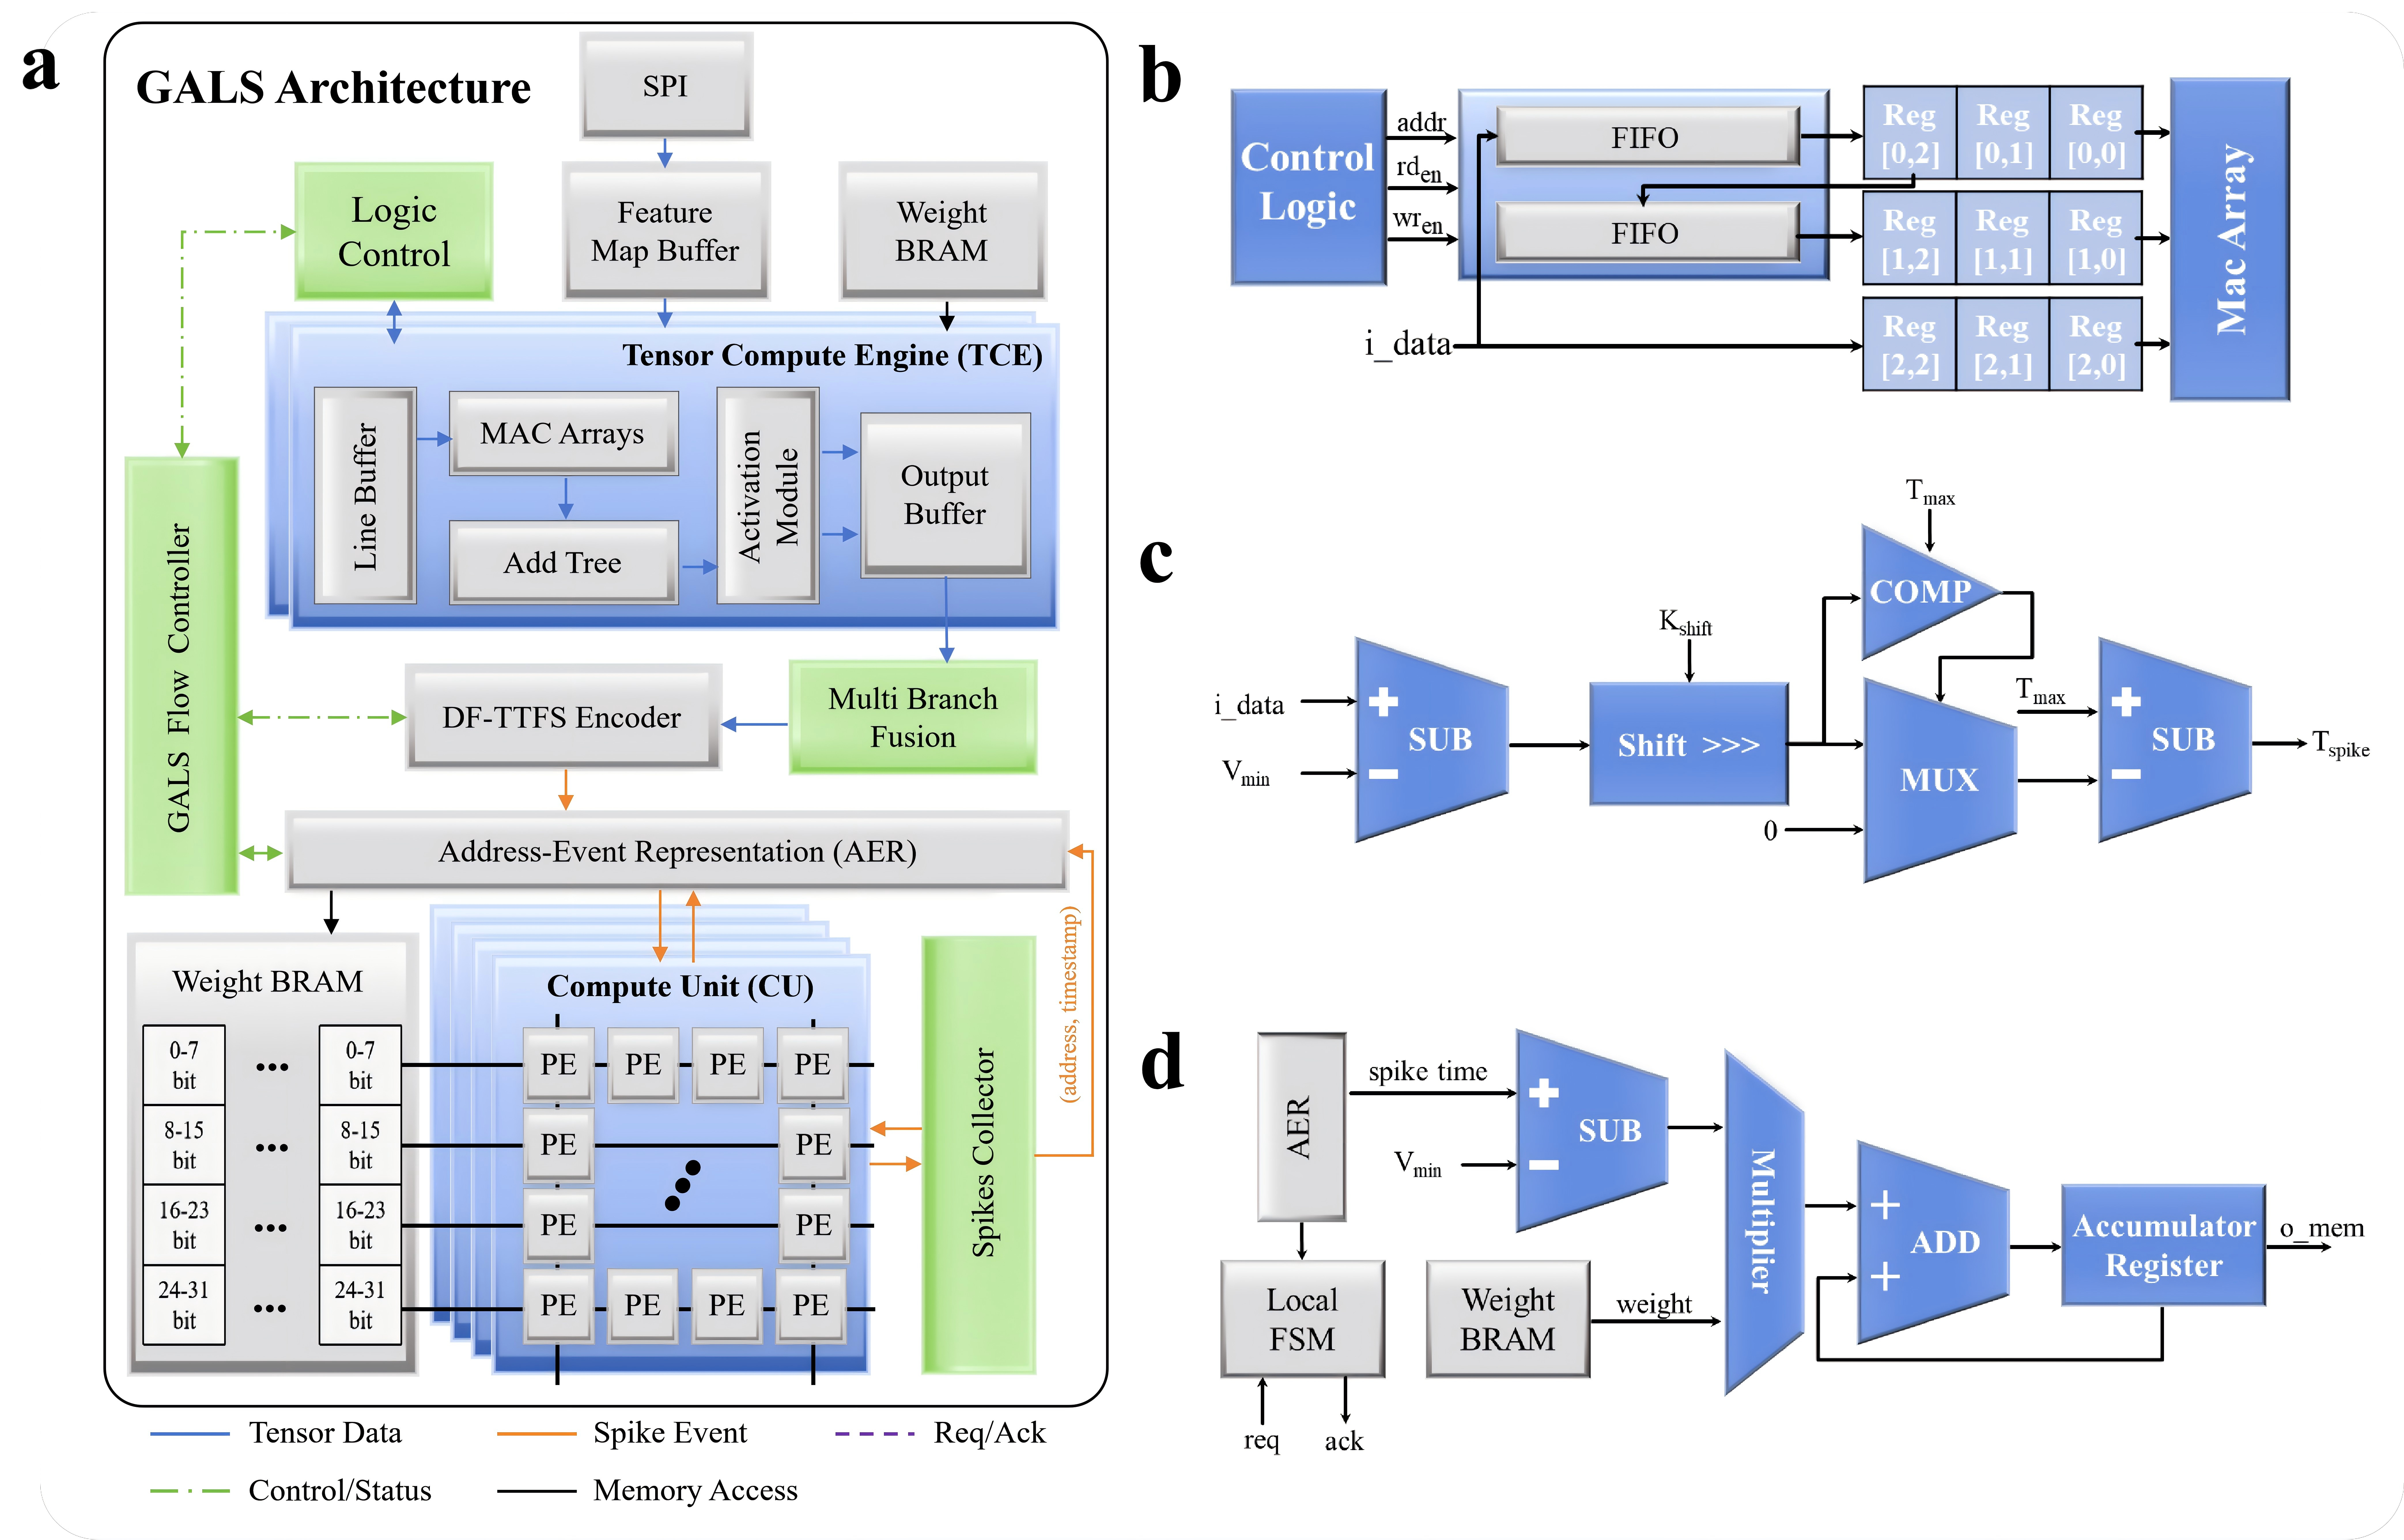
\includegraphics[width=0.95\linewidth]{figures/hardoverview.png}
\end{center}
\noindent\textbf{Fig. 4. Hardware architecture and main components of the proposed accelerator.}
(a) Organization of the globally asynchronous locally synchronous (GALS) accelerator. Blue solid lines trace tensor data from the streaming INT8 tensor compute engine (TCE) to the division-free time-to-first-spike (DF-TTFS) encoder. Orange solid lines trace address-event representation (AER) spike events through the compute unit and processing element (CU/PE) arrays. Each event carries an address and timestamp, and hidden layer events enter the recirculation path. Purple dashed lines denote request/acknowledgment (Req/Ack) handshaking, green dash-dotted lines denote control and status, and thin black lines denote memory access. The tensor pipeline through DF-TTFS belongs to the local \texttt{clk}$_{\mathrm{TCE}}$ island. The weight memory, CU/PE arrays, and spike collector belong to the independent \texttt{clk}$_{\mathrm{SNN}}$ island, with the AER block forming the composite clock domain boundary.
(b) A line buffer implemented with shift registers that continuously reconstructs sliding windows for pipelined convolution.
(c) Hardware implementation of the DF-TTFS encoder using normalization by bit shifts and valid event detection to produce AER spikes.
(d) Microarchitecture of the event-driven PE, showing integration of membrane potentials with time modulation and local clock-enable control. The GALS Flow Controller coordinates start, enable, completion, and layer or array state. It carries only control and status signals, while each island retains its local clock.
}
\EvidenceMainFigFour

\begin{center}
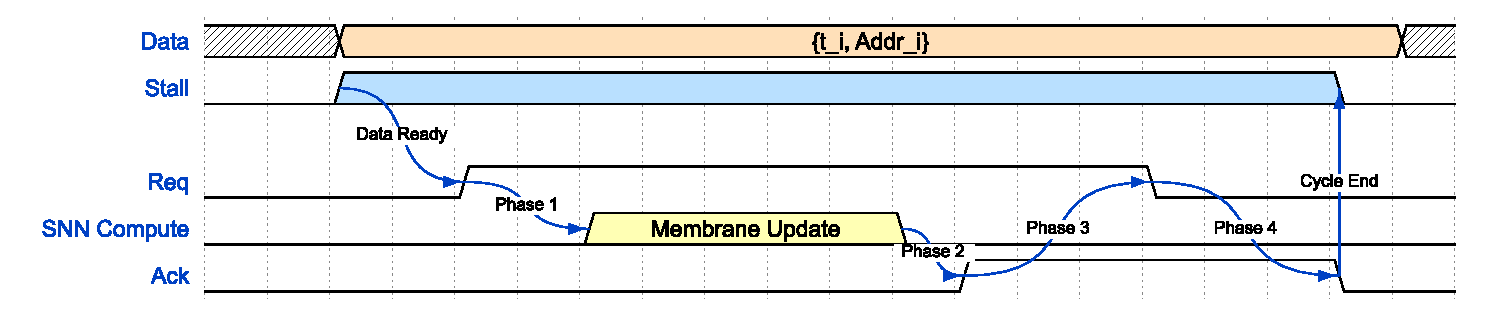
\includegraphics[width=0.98\linewidth]{figures/timingdiagram.eps}
\end{center}
\noindent\textbf{Supplementary Fig. S1.} Timing diagram of the bundled-data four-phase handshake between the locally synchronous \texttt{clk}$_{\mathrm{TCE}}$ and \texttt{clk}$_{\mathrm{SNN}}$ islands. The address/timestamp payload is stabilized before request (Req) assertion and held until synchronized acknowledgment (Ack) completes the transfer.

\vspace{4mm}
\noindent {\bf Comment 1.5:}

``{\it There are also some inconsistencies in terminology. Terms like
``temporal window,'' ``time window,'' and ``spiking window'' are used in
different places without clear distinctions. The model naming is also
not consistent (e.g., DA-SNN, ATSNN, adaptive SNN). In Table 1, metrics
such as Acc, F1, and Spe are reported, but their definitions are not
clearly given in the main text.}''
\vspace{1mm}

\noindent {\bf Response to Comment 1.5:}

We appreciate the careful identification of the terminology and metric inconsistencies. Because they could obscure both the processing stages and the meaning of the reported results, we have assigned one term to each temporal scale and one name to each model scope; we now also define every metric used in the evaluation.

We standardized the terminology throughout the main text and
Supplementary Information. DA-SNN denotes the complete model, whereas
ATSNN denotes its temporal spiking classifier. ``Outer window'' now
refers to EEG segmentation, ``PSE temporal bin'' to the subdivisions
used for feature extraction, and ``layer-wise temporal window'' to the
B1/ATSNN interval; the generic terms ``time window'' and ``spiking
window'' have been replaced where they referred to these defined
objects.

The revised Methods and Supplementary Information define Acc as window-level accuracy, F1 as macro-F1,
and Spe as macro-specificity. Macro-specificity is the unweighted mean
of one-versus-rest specificity across classes. The Supplementary Methods
provide the corresponding formulas, aggregation rules, and
convention for calculating the sample standard deviation.



The standardized definitions appear in \textbf{``Neuromorphic framework for EEG emotion recognition''}, with formulas and aggregation rules in \textbf{Supplementary ``EEG Data Preprocessing'' and ``Evaluation Protocols, Model Selection, and Statistics''}. The input construction is quoted below.

\uline{``Continuous EEG recordings are first z-score normalized and divided into outer windows without overlap. Within each outer window, power spectral entropy (PSE) is calculated over $N_f$ temporally contiguous bins. The electrode values in each bin are projected onto an $H\times W$ topographic grid and stacked to form a dense tensor in $\mathbb{R}^{N_f\times H\times W}$. Thus, the input feature channel axis represents consecutive PSE maps, whereas EEG electrodes occupy positions on the two spatial axes.''}

\vspace{4mm}
\noindent {\bf Comment 1.6:}

``{\it Fig. 4 does not clearly indicate whether the data is represented as
tensors or spike events, which makes the processing pipeline difficult
to follow.}''
\vspace{1mm}

\noindent {\bf Response to Comment 1.6:}

We thank the reviewer for isolating the unclear representation boundary in Fig. 4. We now distinguish the dense INT8 tensor path from the AER event path and identify DF-TTFS as the conversion point.

The revised Fig. 4 legend and accompanying hardware description now
define the representation boundary explicitly. Dense INT8 tensor data
pass through the input buffers, tensor compute engine, multi-branch
fusion path, and DF-TTFS encoder. DF-TTFS is the tensor-to-event
conversion point. Downstream AER packets carry a spike address and
timestamp through the event interface and CU/PE arrays, while
hidden-layer events recirculate through the spike collector and AER
path. The final layer supplies membrane potentials to a comparator-tree
decision unit.



This representation flow is now defined in the \textbf{Fig. 4 legend and ``Hardware Implementation''}; the revised passage is quoted below.

\uline{``The combined streaming and event processing pipeline establishes the accelerator data flow (Fig.~\ref{fig:hardoverview}a). Multichannel data first stream into the on-chip input buffer through a serial peripheral interface (SPI). The reconfigurable tensor compute engine (TCE), multibranch fusion path, and DF-TTFS encoder operate in the local \texttt{clk}$_{\mathrm{TCE}}$ island. A line buffer implemented with shift registers reconstructs sliding windows for pipelined convolution (Fig.~\ref{fig:hardoverview}b), after which the fused INT8 tensor enters DF-TTFS. The encoder forms the representation boundary by converting the dense tensor into sparse AER events. Each event carries an address and timestamp \cite{AER}. The AER block forms a composite interface. Its sending side generates the event and request, while clock domain crossing (CDC) logic transfers the handshake. Routing on the \texttt{clk}$_{\mathrm{SNN}}$ side then delivers the event to the weight memory and CU/PE arrays.''}

\EvidenceMainFigFour

\noindent \textbf{Reference to Comment 1.6:}

\noindent(Note: ``[ ]'' refers to the reference number used in the manuscript or Supplementary Information.)

\noindent[43]\:Boahen KA. ``Point-to-point connectivity between neuromorphic chips using address events.'' In: \textit{IEEE Transactions on Circuits and Systems II: Analog and Digital Signal Processing} 47.5 (2000), pp. 416--434.

\vspace{4mm}
\noindent {\bf Comment 1.7:}

``{\it The introduction provides general background, but the specific research
gap is not stated very clearly. The motivation for combining
asynchronous hardware with EEG-based SNNs could be explained more
directly, especially in relation to existing methods.}''
\vspace{1mm}

\noindent {\bf Response to Comment 1.7:}

We appreciate the reviewer's observation that the original Introduction left the model-to-hardware gap implicit. We have replaced the general motivation with a direct account of why model-level event sparsity requires an execution substrate that also responds to event validity.

We revised the Introduction to state the gap directly while retaining
the original motivation. Affective neural activity motivates event-based
representations, but scalp EEG is continuously sampled and is not itself
a hardware-ready event stream. DA-SNN converts EEG-derived features into
sparse spike events; if those events are still handled by continuously
active synchronous datapaths and memory transfers, part of the
model-level sparsity benefit can be lost. This motivates coupling event
generation in the EEG SNN with a GALS substrate that transfers valid
events between locally synchronous domains and activates the required
data-movement and compute paths.



The revised research gap and design motivation are stated in the \textbf{``Introduction''} as follows.

\uline{``Overall, synchronous acquisition followed by dense computation couples computational cost to the input sampling rate, increasing power and latency as monitoring duration grows. Model compression techniques such as pruning, quantization, and knowledge distillation reduce arithmetic cost \cite{ref25,ref26,ref77}, but dense, globally clocked hardware can still update datapaths at every processed time step. Conversely, sparse model activity yields hardware savings only when data movement and state updates respond to event validity. The unresolved cross-layer problem is therefore to convert features derived from continuously sampled EEG into sparse events and preserve this sparsity through hardware execution.''}

\noindent \textbf{Reference to Comment 1.7:}

\noindent(Note: ``[ ]'' refers to the reference number used in the manuscript or Supplementary Information.)

\noindent[20]\:Han S, Mao H, and Dally WJ. ``Deep Compression: Compressing Deep Neural Networks with Pruning, Trained Quantization and Huffman Coding.'' In: \textit{Proceedings of the International Conference on Learning Representations} (2016).

\noindent[21]\:Jacob B, Kligys S, Chen B, \textit{et al.} ``Quantization and Training of Neural Networks for Efficient Integer-Arithmetic-Only Inference.'' In: \textit{Proceedings of the IEEE Conference on Computer Vision and Pattern Recognition} (2018), pp. 2704--2713.

\noindent[22]\:Gou J, Yu B, Maybank SJ, \textit{et al.} ``Knowledge Distillation: A Survey.'' In: \textit{International Journal of Computer Vision} 129.6 (2021), pp. 1789--1819.

\newpage
\clearpage
\begin{center}
\underline{Responses to Comments of Reviewer 2}
\end{center}
\vspace{3mm}

\vspace{4mm}
\noindent {\bf Comment 2.1:}

``{\it In the efficiency analysis, the hardware comparison is fundamentally
unbalanced. The energy efficiency of the proposed GALS accelerator,
deployed on a customized FPGA, is compared directly against conventional
lightweight CNNs running on a general-purpose ARM processor (Raspberry
Pi 5). This ``apples-to-oranges'' comparison fails to objectively
demonstrate the true architectural advantages of the asynchronous design
against appropriate hardware-level baselines.}''
\vspace{1mm}

\noindent {\bf Response to Comment 2.1:}

We thank the reviewer for insisting on a fair comparison of the GALS clock organization. An FPGA-to-Raspberry-Pi comparison cannot isolate this architectural effect, so we have separated model-level platform comparison from matched hardware evaluation and added two FPGA baselines with clearly defined purposes.

Main Table 2 now presents a model-level comparison on the common
Raspberry Pi 5 platform. To isolate the effect of the clock
organization, we implemented a synchronous version of the same INT8
DA-SNN on the same Zynq-7020 FPGA with the same input tensor and
clock-enable policy; relative to this matched implementation, GALS
increases latency from 16.5 to 18 $\mu$s and adds 172 LUTs and 139 FFs while
reducing total energy from 3.35 to 2.66 $\mu$J per inference. We also
deployed EEGNet on the Zynq-7020: GALS DA-SNN uses more resources and
148 versus 138 mW total power, while reducing latency from 0.772 ms to
18 $\mu$s and energy from 106.536 to 2.66 $\mu$J per inference. The matched
DA-SNN comparison evaluates the clock organization, and EEGNet provides
a cross-model FPGA deployment baseline in Supplementary Table S12.



The revised comparison boundaries are stated in \textbf{Main Table 2, ``Hardware Implementation'', and ``Discussion''}. The matched synchronous implementation and the cross-model EEGNet deployment are detailed in \textbf{Supplementary ``FPGA Deployment Comparisons'' and Table S12}; the main clarification and comparison table are provided below.

\uline{``We additionally implemented a matched synchronous version of the same INT8 DA-SNN on the same FPGA using the same input tensor and clock-enable policy. Relative to this matched implementation, GALS adds 172 LUTs and 139 FFs and increases latency from 16.5 to 18~$\mu$s. Total energy decreases from 3.35 to 2.66~$\mu$J per inference. This comparison isolates the effect of GALS within the implementation.''}

\newcommand{\EvidenceMainTableTwo}{%
\noindent\begin{minipage}{\linewidth}
\smallskip\noindent\textbf{Main Table 2.} Efficiency Analysis of Comparison Classifiers.
\begin{center}
\ResponseTableFormat
\resizebox{\linewidth}{!}{%
\begin{tabular}{@{}lrrrrrr@{}}
\toprule
Model & Params (K) & FLOPs (K) & MACs (K) & \makecell{Parameter\\storage (KB)} & \makecell{Runtime\\memory (KB)} & Power (mW) \\
\midrule
SqueezeNet & 4.12 & 259.97 & 129.98 & 16.09 & 50.43 & 368.33 \\
MobileNetV3-Small & 26.43 & 993.12 & 496.56 & 103.23 & 392.44 & 458.33 \\
MobileNetV3-Large & 543.90 & 9690.00 & 4850.00 & 2119.68 & 3614.72 & 546.35 \\
ShuffleNetV2 & 244.22 & 3490.00 & 1740.00 & 953.98 & 1413.12 & 426.85 \\
EfficientNet-B0 & 1070.00 & 11990.00 & 6000.00 & 4198.40 & 5406.72 & 437.84 \\
EfficientNet-B3 & 1380.00 & 15320.00 & 7660.00 & 5396.48 & 7096.32 & 524.62 \\
Deep ConvNet & 239.48 & 1870.00 & 936.20 & 935.46 & 995.98 & 435.53 \\
Shallow ConvNet & 14.28 & 350.08 & 175.04 & 55.79 & 85.07 & 258.37 \\
EEGNet & 2.72 & 87.55 & 43.78 & 10.64 & 41.04 & 334.86 \\
EESCN & 11080.00 & 308590.00 & 154290.00 & 43284.48 & 225.12 & 776.79 \\
DH-SNN & 152.58 & 476.00 & 235.96 & 587.01 & 260.89 & 236.49 \\
\midrule
\textbf{DA-SNN (FP32)} & 12.76 & 32.47 & 16.23 & 49.83 & 51.27 & 236.68 \\
\textbf{DA-SNN (INT8)} & 12.76 & -- & 16.23 & 12.50 & 13.68 & 184.14 \\
\bottomrule
\end{tabular}%
}
\end{center}
\end{minipage}\par\medskip
}
\EvidenceMainTableTwo

\noindent\begin{minipage}{\linewidth}
\smallskip\noindent\textbf{Supplementary Table S12.} FPGA deployment comparison of the GALS DA-SNN accelerator and EEGNet on Zynq-7020. Energy per inference is calculated from total power and inference latency. The different model architectures and clock targets define this as a deployment comparison; the preceding text provides the matched GALS comparison.
\begin{center}
\ResponseTableFormat
\begin{tabular*}{\linewidth}{@{\extracolsep{\fill}}lcrr@{}}
\toprule
Metric & Unit & GALS DA-SNN & EEGNet \\
\midrule
LUT & count & 10,822 & 6,977 \\
FF & count & 8,164 & 3,097 \\
BRAM & count & 22 & 6 \\
DSP & count & 32 & 5 \\
Clock target & MHz & 100 & 50 \\
Inference latency & $\mu$s & 18 & 772 \\
Dynamic power & mW & 40 & 32 \\
Static power & mW & 108 & 106 \\
Total power & mW & 148 & 138 \\
Total energy/inference & $\mu$J & 2.66 & 106.536 \\
\bottomrule
\end{tabular*}
\end{center}
\end{minipage}\par\medskip
\vspace{4mm}
\noindent {\bf Comment 2.2:}

``{\it Affective EEG signals are highly subject-dependent. While the paper
reports exceptionally high accuracies across datasets, it fails to
explicitly state whether these results are derived from
``within-subject'' or ``cross-subject'' (leave-one-subject-out)
cross-validation. Given the wearable context, the omission of clear
cross-subject generalization metrics is a major empirical flaw.}''
\vspace{1mm}

\noindent {\bf Response to Comment 2.2:}

We appreciate the emphasis on subject-independent evaluation in affective EEG. The original manuscript did not separate overlapping-subject benchmarks from unseen-subject evaluation; we now report these settings independently rather than allowing the high subject-dependent accuracies to imply cross-subject generalization.

Main Table 1 now explicitly reports the subject-dependent random
window-level 80/20 benchmark. The Supplementary Information adds LOSO
evaluation for SEED, SEED-IV, and SEED-V and five fixed subject-holdout
splits for DEAP and DREAMER. Under these subject-independent settings,
DA-SNN ranks first in accuracy, macro-F1, and macro-specificity among
the ten evaluated models on all five datasets.



The distinction is introduced in \textbf{Main Table 1 and ``Emotion Recognition Performance Across EEG Benchmarks''}. Protocol definitions and complete subject-independent results appear in \textbf{Supplementary ``Evaluation Protocols, Model Selection, and Statistics'', ``Subject-Independent Generalization Across EEG Benchmarks'', and Tables S5--S7}; the corresponding main-text statement is quoted below.

\uline{``Table~\ref{tab:overall_15models} compares 15 models on five EEG emotion recognition datasets under a subject-dependent random window-level 80/20 protocol. Subject-independent performance was evaluated separately using leave-one-subject-out (LOSO) for SEED, SEED-IV, and SEED-V and five fixed subject-holdout splits for DEAP and DREAMER (Supplementary Tables~S6 and S7); the corresponding protocols are detailed in the Supplementary Methods.''}

\EvidenceMainTableOne

\providecommand{\EvidenceSuppTableSSix}{%
\smallskip\noindent\textbf{Supplementary Table S6.} Subject-independent leave-one-subject-out (LOSO) performance on the SEED-family datasets. Values are mean $\pm$ sample standard deviation across held-out-subject splits (\%). Acc, window-level accuracy; F1, macro-F1; Spe, macro-specificity. Best results are shown in bold.
\begin{center}
\ResponseTableFormat
\resizebox{\linewidth}{!}{%
\begin{tabular}{@{}lccccccccc@{}}
\toprule
\multirow{2}{*}{Method} & \multicolumn{3}{c}{SEED} & \multicolumn{3}{c}{SEED-IV} & \multicolumn{3}{c}{SEED-V} \\
\cmidrule(lr){2-4}\cmidrule(lr){5-7}\cmidrule(lr){8-10}
& Acc & F1 & Spe & Acc & F1 & Spe & Acc & F1 & Spe \\
\midrule
ShuffleNetV2       & $58.43\pm9.66$ & $56.86\pm10.26$ & $79.25\pm4.81$ & $51.25\pm4.12$ & $48.20\pm4.60$ & $78.71\pm1.37$ & $42.96\pm5.42$ & $38.81\pm4.63$ & $83.30\pm1.26$ \\
Deep ConvNet       & $58.27\pm10.65$ & $54.72\pm12.59$ & $79.14\pm5.36$ & $51.24\pm5.34$ & $46.83\pm7.67$ & $79.13\pm1.89$ & $47.00\pm5.87$ & $39.66\pm8.03$ & $83.14\pm1.66$ \\
MobileNetV3-Small  & $57.08\pm8.48$ & $55.15\pm9.53$ & $78.57\pm4.23$ & $51.23\pm4.16$ & $48.43\pm5.31$ & $78.73\pm1.36$ & $47.36\pm6.13$ & $43.54\pm6.69$ & $83.66\pm1.47$ \\
EEGNet             & $56.69\pm11.00$ & $54.88\pm11.79$ & $78.37\pm5.46$ & $53.82\pm5.52$ & $50.76\pm6.34$ & $79.06\pm1.88$ & $43.32\pm5.17$ & $38.02\pm6.13$ & $82.94\pm1.27$ \\
MobileNetV3-Large  & $56.69\pm8.00$ & $55.34\pm8.26$ & $78.41\pm3.94$ & $50.99\pm3.96$ & $48.01\pm4.92$ & $78.66\pm1.18$ & $41.12\pm5.39$ & $37.80\pm4.97$ & $82.94\pm1.19$ \\
DH-SNN             & $56.36\pm10.03$ & $53.07\pm11.37$ & $78.17\pm5.04$ & $51.95\pm5.07$ & $47.42\pm6.75$ & $78.94\pm1.74$ & $42.29\pm6.07$ & $34.61\pm8.26$ & $82.85\pm1.72$ \\
Shallow ConvNet    & $56.27\pm9.02$ & $51.77\pm10.44$ & $78.13\pm4.55$ & $52.62\pm5.00$ & $43.47\pm6.27$ & $78.27\pm1.78$ & $43.66\pm6.23$ & $32.52\pm8.20$ & $82.47\pm1.79$ \\
EfficientNet-B0    & $55.57\pm9.68$ & $53.37\pm10.04$ & $77.81\pm4.85$ & $50.18\pm3.76$ & $46.76\pm3.89$ & $78.80\pm1.27$ & $43.93\pm4.50$ & $38.29\pm5.25$ & $82.80\pm1.10$ \\
SqueezeNet         & $36.88\pm8.95$ & $22.13\pm14.29$ & $68.34\pm4.50$ & $45.78\pm3.04$ & $29.27\pm2.52$ & $75.00\pm1.06$ & $38.81\pm4.03$ & $21.80\pm3.01$ & $80.00\pm1.07$ \\
\textbf{DA-SNN}   & $\mathbf{59.10\pm6.93}$ & $\mathbf{57.60\pm7.18}$ & $\mathbf{80.00\pm3.47}$ & $\mathbf{55.80\pm4.55}$ & $\mathbf{52.40\pm5.76}$ & $\mathbf{79.80\pm1.53}$ & $\mathbf{48.20\pm4.50}$ & $\mathbf{44.40\pm5.60}$ & $\mathbf{84.30\pm1.19}$ \\
\bottomrule
\end{tabular}%
}
\end{center}
}
\EvidenceSuppTableSSix

\providecommand{\EvidenceSuppTableSSeven}{%
\smallskip\noindent\textbf{Supplementary Table S7.} Cross-subject performance on DEAP and DREAMER using five fixed subject-holdout splits. Values are mean $\pm$ sample standard deviation across splits (\%). Acc, window-level accuracy; F1, macro-F1; Spe, macro-specificity. Best results are shown in bold.
\begin{center}
\ResponseTableFormat
\resizebox{\linewidth}{!}{%
\begin{tabular}{@{}lcccccc@{}}
\toprule
\multirow{2}{*}{Method} & \multicolumn{3}{c}{DEAP: 26 train/6 held-out subjects} & \multicolumn{3}{c}{DREAMER: 19 train/4 held-out subjects} \\
\cmidrule(lr){2-4}\cmidrule(lr){5-7}
& Acc & F1 & Spe & Acc & F1 & Spe \\
\midrule
MobileNetV3-Large & $52.49\pm3.91$ & $32.27\pm5.96$ & $75.31\pm6.96$ & $61.81\pm3.29$ & $38.32\pm2.87$ & $76.26\pm1.48$ \\
DH-SNN            & $51.26\pm4.64$ & $32.51\pm4.91$ & $75.63\pm7.63$ & $60.14\pm6.52$ & $31.51\pm2.95$ & $75.19\pm0.43$ \\
ShuffleNetV2      & $51.22\pm5.30$ & $30.41\pm1.89$ & $75.24\pm1.26$ & $59.63\pm3.54$ & $35.47\pm5.72$ & $75.40\pm7.75$ \\
Deep ConvNet      & $52.47\pm4.96$ & $31.62\pm2.90$ & $75.12\pm2.01$ & $60.57\pm5.84$ & $34.08\pm5.38$ & $76.06\pm1.24$ \\
Shallow ConvNet   & $52.68\pm5.31$ & $30.68\pm1.73$ & $75.11\pm0.93$ & $59.90\pm5.89$ & $31.27\pm1.80$ & $75.33\pm5.02$ \\
EfficientNet-B0   & $51.16\pm5.33$ & $30.04\pm2.77$ & $75.17\pm2.35$ & $60.34\pm6.60$ & $31.69\pm4.93$ & $75.90\pm1.80$ \\
EEGNet            & $50.94\pm4.79$ & $31.31\pm2.96$ & $75.13\pm2.58$ & $58.36\pm4.57$ & $39.16\pm5.56$ & $76.57\pm1.46$ \\
MobileNetV3-Small & $51.92\pm5.20$ & $32.88\pm2.18$ & $75.30\pm4.25$ & $58.04\pm5.07$ & $35.13\pm5.28$ & $75.53\pm4.67$ \\
SqueezeNet        & $43.90\pm8.67$ & $24.71\pm2.69$ & $75.00\pm4.67$ & $61.48\pm6.06$ & $33.33\pm2.12$ & $75.41\pm4.62$ \\
\textbf{DA-SNN}  & $\mathbf{54.30\pm4.80}$ & $\mathbf{35.60\pm3.40}$ & $\mathbf{76.30\pm2.83}$ & $\mathbf{64.80\pm5.15}$ & $\mathbf{43.40\pm3.95}$ & $\mathbf{77.20\pm1.29}$ \\
\bottomrule
\end{tabular}%
}
\end{center}
}
\EvidenceSuppTableSSeven

\vspace{4mm}
\noindent {\bf Comment 2.3:}

``{\it The methodology relies heavily on Linear Dynamical System (LDS)
smoothing to filter the feature sequences across windows. LDS smoothing
inherently requires observing sequences over time, which introduces
significant computational latency, memory buffering, and complex matrix
operations. The manuscript entirely fails to address how this
computationally expensive, latency-inducing smoothing process is
executed in real-time on the proposed resource-constrained edge
hardware. Ignoring the front-end preprocessing cost renders the
``real-time wearable'' deployment claims highly questionable.}''
\vspace{1mm}

\noindent {\bf Response to Comment 2.3:}

We are grateful for the opportunity to correct a necessary boundary in the original efficiency claim. Accelerator latency is not equivalent to acquisition-to-decision latency when PSE extraction and trial-wise LDS smoothing are performed upstream, and we now state this boundary explicitly.

The reported 18 $\mu$s latency and 2.66 $\mu$J energy cover accelerator
inference from a preprocessed input tensor to the class output; PSE
extraction and trial-wise LDS smoothing are outside this measurement. We
implemented and measured PSE and LDS as independent kernels on the same
FPGA board. PSE requires 10.25 ms and 1,158.25 $\mu$J for one
200-sample call; LDS requires 0.216 ms and 23.544 $\mu$J for 288 lanes
over three test steps (864 outputs). These kernels and the accelerator
were tested independently, so their static power and energy values
cannot be added to claim an integrated end-to-end result. We have
therefore restricted the real-time claim to accelerator inference and
state explicitly that acquisition-to-decision latency and energy remain
to be measured in an integrated wearable system.



We now state this measurement boundary in \textbf{``Hardware Implementation'', ``Discussion'', and ``Conclusion''}. The boundary is defined directly in \textbf{Supplementary ``Hardware Measurement Boundary and Standalone Preprocessing Kernels''}, and the standalone kernel measurements are reported in \textbf{Supplementary Table S9}; the revised boundary statement and measured table are included below.

\uline{``The reported 18~$\mu$s latency and 40/108/148~mW dynamic/static/total power describe one accelerator inference from a preprocessed input tensor to the class output. The board power measurement uses the programmable logic (PL) accelerator boundary. It includes on-chip input and feature buffers, the PL serial peripheral interface (SPI), tensor compute engine (TCE), multibranch fusion path, DF-TTFS encoder, valid event filtering, AER/CDC interface, weight memory, CU/PE arrays, spike collector, controller, and final decision logic. EEG acquisition, PSE extraction, LDS smoothing within each trial, processing system (PS) cores, external double data rate (DDR) memory, and board peripherals lie outside this boundary. Thus, the reported 18~$\mu$s latency, 148~mW total power, and 2.66~$\mu$J energy apply only to the FPGA accelerator components listed as included above; PSE and LDS are characterized separately below.''}

\newcommand{\EvidenceSuppTableSNine}{%
\noindent\begin{minipage}{\linewidth}
\smallskip\noindent\textbf{Supplementary Table S9.} Standalone FPGA measurements of preprocessing kernels at board level. PSE, LDS, and the GALS accelerator were tested independently, and each power and energy value retains its own measurement boundary. Power components were rounded independently.
\begin{center}
\ResponseTableFormat
\resizebox{\linewidth}{!}{%
\begin{tabular}{@{}lrrrrclrrrrr@{}}
\toprule
Kernel & LUT & FF & BRAM & DSP & \makecell{Clock\\(MHz)} & Workload & \makecell{Latency\\(ms)} & \makecell{Dynamic power\\(mW)} & \makecell{Static power\\(mW)} & \makecell{Total power\\(mW)} & \makecell{Energy\\($\mu$J)} \\
\midrule
PSE & 13,550 & 479 & 34 & 44 & 2 & one 200-sample call & 10.25 & 7 & 106 & 113 & 1,158.25 \\
LDS & 4,797 & 374 & 1 & 8 & 4 & 288 lanes $\times$ 3 steps & 0.216 & 5 & 105 & 109 & 23.544 \\
\bottomrule
\end{tabular}%
}
\end{center}
\end{minipage}\par\medskip
}
\EvidenceSuppTableSNine
\vspace{4mm}
\noindent {\bf Comment 2.4:}

``{\it The authors acknowledge in the Discussion that long-term wearable
deployment faces severe challenges from individual state variations and
electrode impedance drift. However, for a system whose primary selling
point is enabling ``continuous wearable monitoring,'' the complete
absence of any implemented online adaptive or calibration mechanism is a
critical functional gap in the proposed framework.}''
\vspace{1mm}

\noindent {\bf Response to Comment 2.4:}

We appreciate the reviewer pressing us to state the absence of online calibration as a limitation. This is a genuine constraint for continuous long-term use: the present implementation is a fixed-parameter inference prototype, not an online-learning or self-calibrating wearable system.

The current prototype uses fixed parameters trained offline and does not
implement online learning or recalibration. We therefore do not present
the revision as resolving long-term subject or electrode drift, and we
have narrowed the deployment claim to a fixed-parameter inference
prototype. The Discussion and Conclusion now identify session-level
calibration and selective parameter adaptation as necessary future
extensions whose storage, update logic, and energy costs require
separate evaluation.

This scope and the required next steps are now stated explicitly in the \textbf{``Discussion'' and ``Conclusion''}; the revised limitation reads as follows.

\uline{``The present study evaluates an inference architecture with parameters fixed after training. Although the subject-independent protocols measure generalization to held-out subjects, longitudinal changes and subject-specific adaptation during prolonged use remain to be studied. The perturbation experiments use models trained separately for each synthetic noise condition. Evaluation on wearable recordings is therefore needed to characterize motion, electromyographic (EMG), electrooculographic (EOG), electrode-contact, impedance, and sweat artifacts.''}

\uline{``Future work should measure acquisition-to-decision latency, total memory, energy, and stability during continuous operation, and should evaluate session calibration or selective parameter adaptation together with their storage, update logic, and energy costs.''}

\vspace{4mm}
\noindent {\bf Comment 2.5:}

``{\it The Globally Asynchronous Locally Synchronous (GALS) architecture relies
on a complex four-phase handshake protocol and Address-Event
Representation (AER) routing to cross clock domains. The authors praise
the energy reduction from sparse compute activation but completely
ignore the significant dynamic power, physical area footprint, and
latency overhead inherently introduced by the AER routing logic,
threshold filters, and metastability-prevention synchronizers. Without a
transparent, component-level breakdown of the GALS interface overhead,
the isolated 40 mW dynamic power figure is incomplete and highly
misleading.}''
\vspace{1mm}

\noindent {\bf Response to Comment 2.5:}

We thank the reviewer for requesting a transparent accounting of the AER/CDC interface. Sparse activation does not make this interface free; routing, filtering, synchronization, and handshake logic incur resource and latency costs and must remain inside the efficiency assessment.

The revised manuscript provides an interface breakdown covering
event-valid filtering, AER routing, address decoding, Req/Ack
synchronizers, four-phase handshake state machines, and clock-enable
control. Because some of this logic has functional counterparts in the
synchronous design, the matched implementation gives the relevant net
overhead: GALS adds 172 LUTs and 139 FFs and increases latency from 16.5
to 18 $\mu$s (9.09\%). The
reported 40 mW dynamic power includes the complete interface but cannot
be partitioned reliably by synthesis hierarchy; we now state this
limitation instead of assigning an unsupported component-level power
percentage. At the complete-design level, the matched synchronous
implementation consumes 96 mW dynamic power and 3.35 $\mu$J per
inference, compared with 40 mW and 2.66 $\mu$J for GALS.



The complete accounting is now distributed across \textbf{``Hardware Implementation'' and ``Discussion''} and \textbf{Supplementary ``Detailed Hardware Control Protocol'', ``Hardware Measurement Boundary and Standalone Preprocessing Kernels'', ``FPGA Resource Utilization and GALS Interface Cost'', ``FPGA Deployment Comparisons'', ``FPGA Latency and Energy Measurement'', and Tables S9--S11 and S13}. The interface boundary and hierarchical breakdown are provided below.

\uline{``The GALS interface consumes logic and adds transfer latency. It includes valid event filtering, AER routing and broadcasting, hidden layer recirculation, address decoding, synchronizers with two stages in both directions, four-phase handshake state machines, and clock-enable control. Each accepted event therefore incurs routing and protocol work even in a sparse stream. Hierarchical synthesis of the complete design resolves the LUT and flip-flop counts and functional latencies reported below. Dynamic power remains aggregated for the complete accelerator, so the analysis assigns no separate power percentage to an interface component.''}

\noindent\begin{minipage}{\linewidth}
\smallskip\noindent\textbf{Supplementary Table S10.} FPGA resource utilization of the complete GALS accelerator.
\begin{center}
\ResponseTableFormat
\begin{tabular*}{\linewidth}{@{\extracolsep{\fill}}lrrr@{}}
\toprule
Resource & Used & Available & Utilization (\%) \\
\midrule
LUT & 10,822 & 53,200 & 20.34 \\
FF & 8,164 & 106,400 & 7.67 \\
BRAM & 22 & 140 & 15.71 \\
DSP & 32 & 220 & 14.55 \\
\bottomrule
\end{tabular*}
\end{center}
\end{minipage}\par\medskip

\noindent\begin{minipage}{\linewidth}
\smallskip\noindent\textbf{Supplementary Table S11.} Hierarchical synthesis breakdown of logic associated with the GALS interface. Functional latencies describe individual blocks and are reported separately; the matched comparison in the text reports the net resource difference.
\begin{center}
\ResponseTableFormat
\begin{tabular*}{\linewidth}{@{\extracolsep{\fill}}lrrl@{}}
\toprule
Component & LUT & FF & Functional latency \\
\midrule
Threshold/event-valid filter & 93 & 42 & 1 cycle \\
AER arbitration/router & 512 & 286 & 2 cycles \\
Address decoder & 148 & 79 & 1 cycle \\
Req/Ack synchronizers & 26 & 36 & 3 destination-clock cycles per crossing \\
Four-phase handshake FSM & 87 & 53 & 11 cycles per complete handshake \\
Clock-enable controller & 115 & 106 & 1 cycle \\
Complete GALS accelerator & 10,822 & 8,164 & 18~$\mu$s per inference \\
\bottomrule
\end{tabular*}
\end{center}
\end{minipage}\par\medskip

\newcommand{\EvidenceSuppTableSThirteen}{%
\noindent\begin{minipage}{\linewidth}
\smallskip\noindent\textbf{Supplementary Table S13.} GALS FPGA latency, power, and energy within the accelerator inference boundary.
\begin{center}
\ResponseTableFormat
\begin{tabular*}{\linewidth}{@{\extracolsep{\fill}}lrr@{}}
\toprule
Metric & Value & Unit \\
\midrule
Latency & 18 & $\mu$s \\
Dynamic power & 40 & mW \\
Static power & 108 & mW \\
Total power & 148 & mW \\
Dynamic energy/inference & 0.72 & $\mu$J \\
Total energy/inference & 2.66 & $\mu$J \\
\bottomrule
\end{tabular*}
\end{center}
\end{minipage}\par\medskip
}
\EvidenceSuppTableSThirteen
\vspace{4mm}
\noindent {\bf Comment 2.6:}

``{\it There is a highly noticeable and strange inconsistency in the
manuscript's formatting. Specifically, Table 1 and Table 2 are
completely different in size, scale, and layout. This glaring visual
discrepancy looks highly unprofessional and severely disrupts the
reading experience.}''
\vspace{1mm}

\noindent {\bf Response to Comment 2.6:}

We appreciate the reviewer's attention to the inconsistent presentation of the two main tables. We have harmonized their styling while retaining the width difference required by their substantially different information densities.

We revised both main tables to use the same typographic language:
booktabs rules without vertical lines or shading, consistent caption
style, unit placement in column headers, abbreviation definitions,
numeric precision, and restrained boldface. Table 1 remains wider
because it reports 15 metrics across five datasets, whereas Table 2
remains a compact efficiency table; the difference in information
density no longer produces unrelated styling.



The revised styling is applied to \textbf{Main Tables 1 and 2}.

The restored Table 2 title is:

\uline{``Efficiency Analysis of Comparison Classifiers.''}

\EvidenceMainTableOne
\EvidenceMainTableTwo

\newpage
\clearpage
\begin{center}
\underline{Responses to Comments of Reviewer 3}
\end{center}
\vspace{3mm}

\vspace{4mm}
\noindent {\bf Comment 3.1:}

``{\it The manuscript reports only average performance metrics across datasets,
without providing measures of variability such as standard deviation.
Considering the inherent variability in EEG signals across subjects and
trials, including statistical dispersion would improve the credibility
and robustness of the reported results.}''
\vspace{1mm}

\noindent {\bf Response to Comment 3.1:}

We thank the reviewer for the statistical recommendation to report variability across repeated runs and subject-independent splits. Point estimates alone do not reveal this variability, so we have added dispersion measures while keeping the aggregation unit explicit for each evaluation protocol.

Main Table 1 and the cross-dataset ablations now report DA-SNN results
as mean $\pm$ sample standard deviation across random seeds 1--5. The
SEED-family LOSO tables report mean $\pm$ sample standard deviation across
held-out subjects. For DEAP and DREAMER, Supplementary Table S7 reports
mean $\pm$ sample standard deviation across five fixed subject-holdout
splits, using 26/6 and 19/4 train/held-out subjects, respectively. These
summaries quantify seed, held-out-subject, or
held-out-subject-composition variability; trial-level dispersion was not
estimated separately.



The aggregation conventions are defined in the \textbf{Supplementary ``Evaluation Protocols, Model Selection, and Statistics''}. The resulting variability estimates appear in \textbf{Supplementary ``Subject-Independent Generalization Across EEG Benchmarks'', ``Ablation Studies'', and Tables S6--S8}; the revised statistical definition is quoted below.

\uline{``Accuracy is the proportion of correctly classified held-out windows. Macro-F1 is the unweighted mean of the F1 scores for each class. Macro-specificity treats each class in a one-versus-rest manner. For each class, specificity is calculated as $\mathrm{TN}/(\mathrm{TN}+\mathrm{FP})$ from true negatives (TN) and false positives (FP), followed by an unweighted mean across classes. When measurements for repeats or splits were available, we report the arithmetic mean and sample standard deviation (\texttt{ddof} = 1). Main Table~1 reports DA-SNN as mean $\pm$ sample standard deviation across repeated runs, while baseline point estimates are retained as available. The SEED family LOSO results are reported as mean $\pm$ sample standard deviation across splits of held-out subjects. The DEAP and DREAMER results are reported as mean $\pm$ sample standard deviation across the five predefined subject-holdout splits.''}

\EvidenceMainTableOne
\EvidenceSuppTableSSix
\EvidenceSuppTableSSeven
\EvidenceSuppTableSEight

\vspace{4mm}
\noindent {\bf Comment 3.2:}

``{\it The manuscript uses terms such as ``temporal window,'' ``time window,''
and ``spiking window'' interchangeably without clearly distinguishing
their meanings. In addition, the model naming (e.g., DA-SNN, ATSNN,
adaptive SNN) is not consistent throughout the paper, which may lead to
confusion. A more consistent use of terminology would improve the
overall readability.}''
\vspace{1mm}

\noindent {\bf Response to Comment 3.2:}

We appreciate this careful reading of the terminology. The reviewer identifies two related sources of ambiguity: several temporal scales shared overlapping names, and model-level and classifier-level names were used interchangeably. We have standardized both naming systems.

We standardized the terminology across the main text and Supplementary
Information. DA-SNN denotes the complete architecture, and ATSNN denotes
its temporal spiking classifier. We use ``outer window'' for EEG
segmentation, ``PSE temporal bin'' for feature-extraction subdivisions,
and ``layer-wise temporal window'' for the B1/ATSNN interval; the
generic names ``adaptive SNN'', ``time window'', and ``spiking window''
have been replaced where they referred to these defined objects.



The model names are now fixed in \textbf{``Neuromorphic framework for EEG emotion recognition'' and Fig. 2}, while the three temporal scales are defined in \textbf{Supplementary ``EEG Data Preprocessing'', ``B1 Model Definition and Forward Semantics'', and ``Local Weight Gradient Relation and Adaptive Temporal Window Regulation''}. The defining passage is quoted below.

\uline{``The model then maps this dense EEG-derived tensor to a sparse spike-time representation. As shown in Fig.~\ref{fig:DA-SNN}, DA-SNN processes the tensor through DSGM for gated feature extraction, division-free TTFS encoding \cite{TTFS}, and an adaptive temporal spiking neural network (ATSNN) for classification. DSGM operates on dense-valued feature tensors; DF-TTFS defines the tensor-to-event boundary by mapping refined activations to spike times before spiking inference.''}

\newcommand{\EvidenceMainFigTwo}{%
\begin{center}
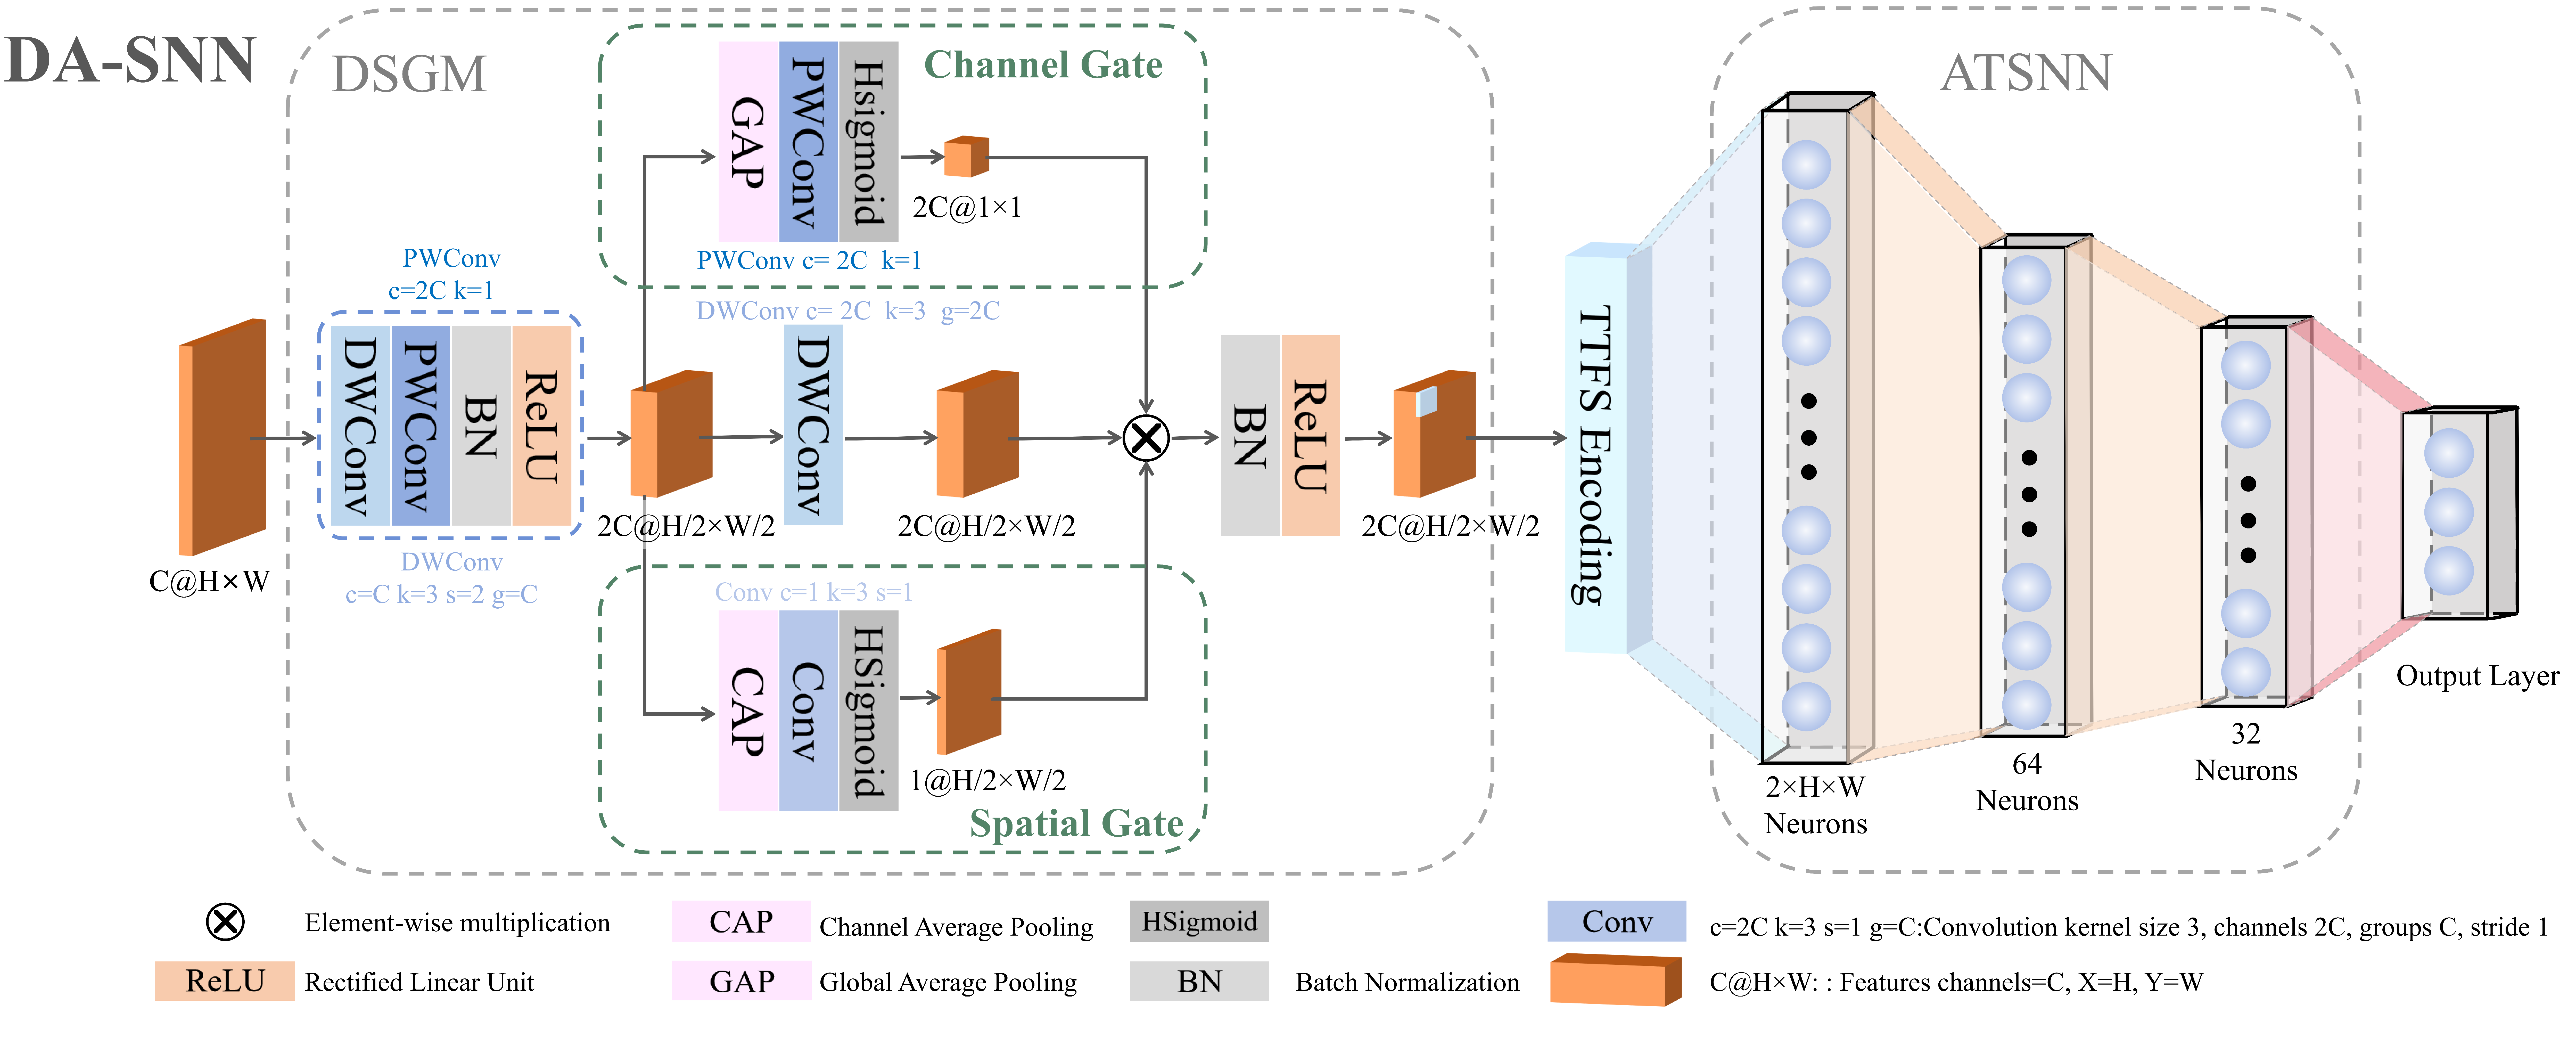
\includegraphics[width=0.98\linewidth]{figures/DA-SNN.eps}
\end{center}
\noindent\textbf{Fig. 2. The proposed DA-SNN model framework.}
The input is a dense tensor derived from EEG, with temporally contiguous power spectral entropy maps along the feature channel axis and the topographic electrode grid along the two spatial axes. DSGM combines depthwise separable feature extraction with channel and spatial gating. DF-TTFS preserves the tensor shape while converting the DSGM output into spike times for ATSNN classification. The circled multiplication symbol denotes the Hadamard product, and $C@H\times W$ specifies the number of feature channels and the spatial dimensions. DWConv, depthwise convolution; PWConv, pointwise convolution; GAP, global average pooling; CAP, channel average pooling; BN, batch normalization; HSigmoid, Hard-Sigmoid; DF-TTFS, division-free time-to-first-spike; ATSNN, adaptive temporal spiking neural network. Spatial dimensions are shown schematically; dataset-specific dimensions, convolution parameters, and broadcasting rules are provided in the Supplementary Information.
}
\EvidenceMainFigTwo

\noindent \textbf{Reference to Comment 3.2:}

\noindent(Note: ``[ ]'' refers to the reference number used in the manuscript or Supplementary Information.)

\noindent[30]\:Thorpe S, Delorme A, and Van Rullen R. ``Spike-Based Strategies for Rapid Processing.'' In: \textit{Neural Networks} 14.6--7 (2001), pp. 715--725.

\vspace{4mm}
\noindent {\bf Comment 3.3:}

``{\it Although the manuscript presents results under different conditions
(e.g., noise or quantization), these evaluations are not compared
against a clear reference baseline under the same settings. Including a
simple baseline curve would make the robustness claims more convincing
and easier to interpret.}''
\vspace{1mm}

\noindent {\bf Response to Comment 3.3:}

We are grateful for the suggestion to include matched references in the perturbation analysis. The original curves could not show whether the observed degradation was specific to DA-SNN or common across models, so we redesigned the experiment around two baselines evaluated under the same generated perturbations and training protocol.

We redesigned Fig. 3a to compare DA-SNN with DH-SNN and EEGNet under
matched perturbation conditions on SEED, DEAP, and DREAMER. Within each
condition, the models use the same generated noisy data bundle, random
window-level 80/20 split, model seed, training schedule,
checkpoint-selection rule, and evaluation level. The revised analysis
covers Gaussian noise, low-frequency drift, and EMG-like transient
bursts at NL values from 0.01 to 0.125, together with the clean
condition.

Because the analysis uses noise-matched retraining rather than a
fixed clean-trained checkpoint, the curves are interpreted descriptively
and no statistical significance or zero-shot robustness is claimed. For
Fig. 3b, the full-precision 32-bit DA-SNN serves as the matched reference
because this panel addresses a deployment-design question: selecting the
weight precision that best balances accuracy retention and hardware
resource cost. We therefore compare the same DA-SNN at 16, 12, 8, 6,
and 4 bits against its 32-bit reference. This within-model trade-off
identifies 8-bit precision as the deployment operating point, while the
cross-model robustness comparison is provided separately in Fig. 3a.



The matched robustness comparison and its interpretation are reported in \textbf{Fig. 3a and ``Sensitivity to Controlled EEG Perturbations and Quantization''}, with the generation and training details in \textbf{Supplementary ``Controlled EEG Perturbation Protocol''}. The same Results section explains that \textbf{Fig. 3b} is used to select the deployment bit width by balancing accuracy and hardware resource requirements. The revised Results passages and figure are included below.

\uline{``We assessed sensitivity to controlled signal corruption on SEED, DEAP, and DREAMER using additive Gaussian noise, low-frequency drift, and EMG-like transient bursts (Fig.~\ref{fig:robust_quant_comparison}a). Each perturbation was applied to time-domain EEG samples after dataset-specific signal conditioning and segmentation but before PSE extraction, spatial mapping, and LDS smoothing. The relative noise level was defined per channel as $\mathrm{NL}=\sigma_{\mathrm{noise}}/\sigma_{\mathrm{signal}}$ and varied over $\{0.01,0.03,0.05,0.08,0.10,0.125\}$. DA-SNN, DH-SNN, and EEGNet were trained and evaluated for each noise condition using the same random window-level 80/20 protocol.''}

\uline{``At $\mathrm{NL}=0.125$, the accuracy decrease from clean data ranged from 3.71 to 9.37 percentage points for DA-SNN across the nine dataset--perturbation combinations, compared with 7.13--15.61 points for DH-SNN and 5.09--11.40 points for EEGNet.''}

\uline{``We further examined sensitivity to weight quantization by reducing the precision of floating-point weights from 32 to 16, 12, 8, 6, and 4 bits using quantization-aware training (Fig.~\ref{fig:robust_quant_comparison}b). Accuracy was $96.98\%$ at 32 bits and $96.94\%$ at 8 bits, before decreasing to $95.37\%$ at 6 bits and $77.81\%$ at 4 bits. We therefore selected 8-bit weights for deployment. The integer model uses signed INT8 weights and unsigned 8-bit nonnegative activations, as detailed in the Supplementary Information.''}

\newcommand{\EvidenceMainFigThree}{%
\begin{center}
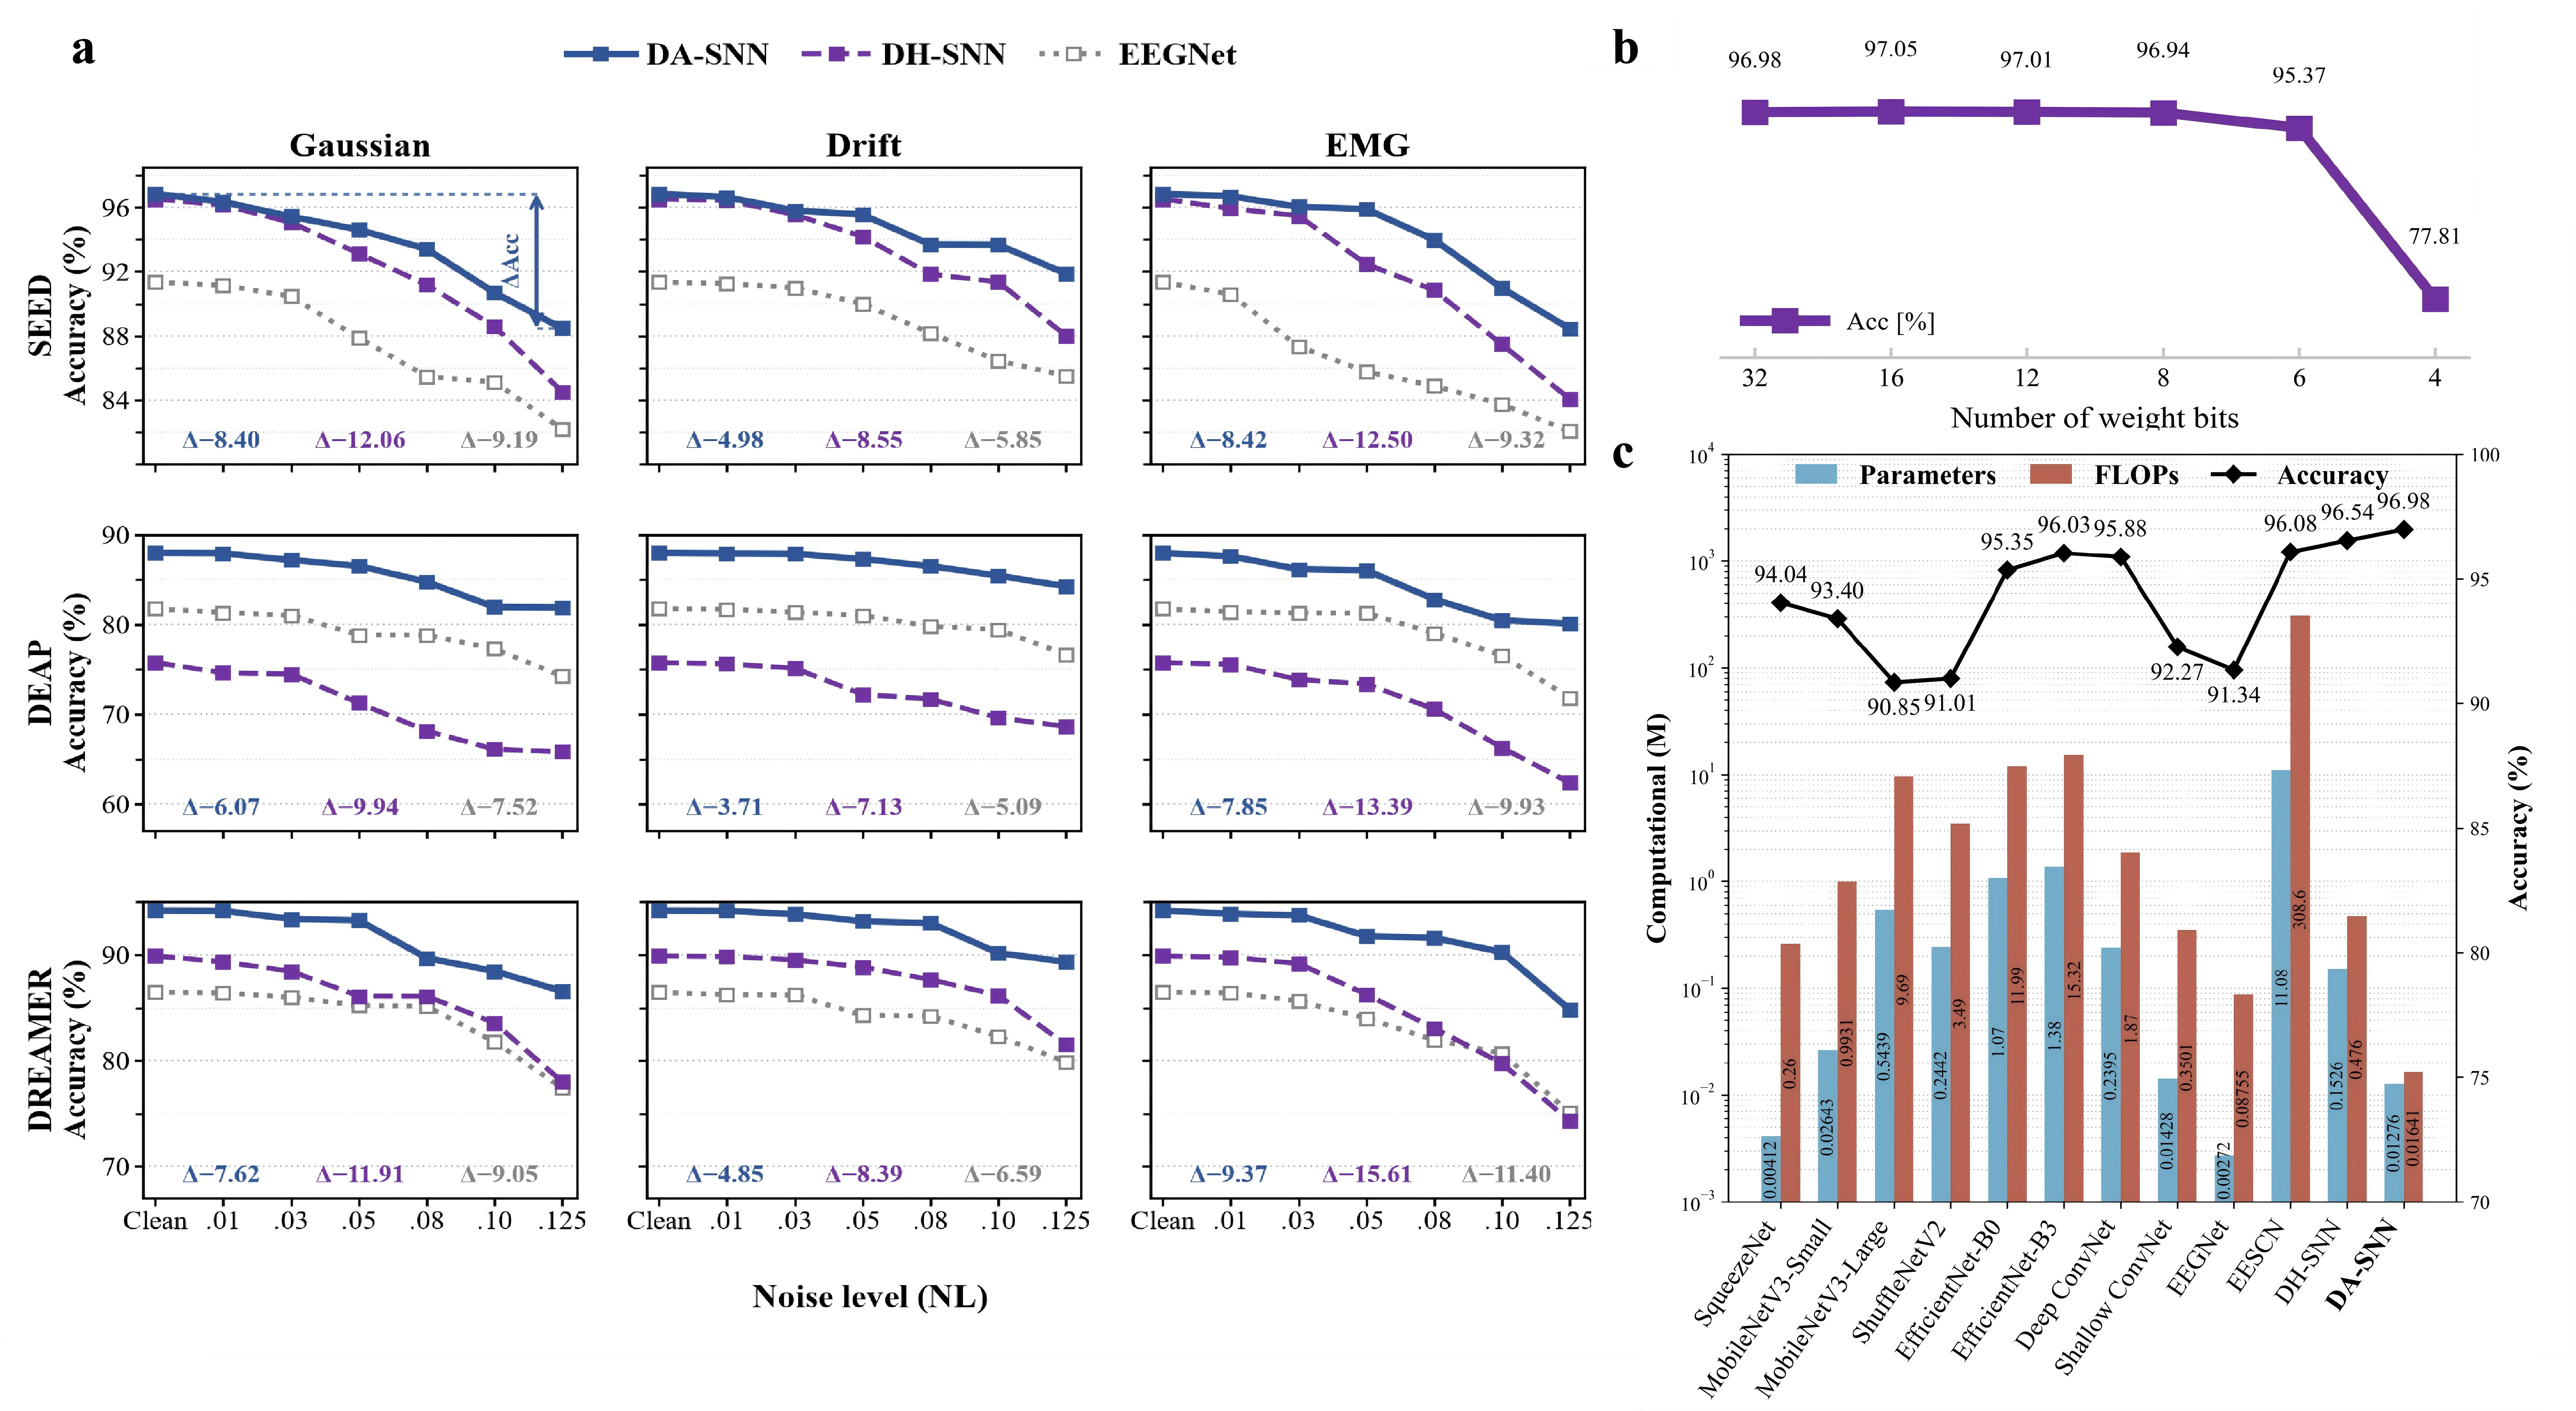
\includegraphics[width=0.98\linewidth]{figures/robustness_quantization_comparison.png}
\end{center}
\noindent\textbf{Fig. 3. Sensitivity to controlled EEG perturbations, weight quantization, and model complexity.}
\textbf{(a)} Accuracy of DA-SNN, DH-SNN, and EEGNet on SEED, DEAP, and DREAMER under Gaussian noise, low-frequency drift, and electromyographic (EMG)-like transient bursts. Perturbations were added to time-domain EEG samples before PSE extraction, spatial mapping, and LDS smoothing. Relative noise level (NL) denotes the ratio of the perturbation standard deviation to the clean signal standard deviation within each channel; Clean denotes $\mathrm{NL}=0$. Endpoint annotations report $\Delta\mathrm{Acc}=\mathrm{Acc}_{\mathrm{NL}=0.125}-\mathrm{Acc}_{\mathrm{Clean}}$ in percentage points.
\textbf{(b)} SEED accuracy in a weight-bit-width sweep from 32 to 4 bits using quantization-aware training.
\textbf{(c)} Performance comparison of DA-SNN with representative lightweight models. FLOPs and parameter counts are normalized.
}
\EvidenceMainFigThree

\vspace{4mm}
\noindent {\bf Comment 3.4:}

``{\it While the overall pipeline is described, the connection between the
continuous EEG features, the encoding process, and the spiking neural
network is not sufficiently detailed. Providing a clearer description of
data transformations at each stage would improve the understanding of
the end-to-end system.}''
\vspace{1mm}

\noindent {\bf Response to Comment 3.4:}

We thank the reviewer for requesting a representation-level account of the pipeline. The original description did not track the representation at each stage; we now state explicitly how continuous EEG becomes a dense spatial--spectral tensor and where that tensor is converted into spike times.

We added a stepwise representation description. Continuous EEG is
z-score normalized and divided into non-overlapping outer windows; PSE
is calculated in temporally contiguous bins; electrode values are
projected to a topographic grid; and the maps are stacked into a dense
tensor in \(\mathbb{R}^{N_f\times H\times W}\). DSGM refines this dense
tensor, and DF-TTFS then defines the dense-to-event boundary by mapping
it to a shape-matched spike-time representation for ATSNN
classification.



The two figures now have distinct roles. \textbf{Fig. 1} provides the system-level route from continuous EEG preprocessing to DA-SNN inference and hardware deployment; it is cited in the revised opening paragraph only to orient the complete pipeline. \textbf{Fig. 2} provides the model-level detail, showing the dense tensor through DSGM and the DF-TTFS tensor-to-spike-time boundary before ATSNN. The corresponding modifications are located in \textbf{``Neuromorphic framework for EEG emotion recognition'' and the Fig. 2 legend}, with dataset-specific tensor construction in \textbf{Supplementary ``EEG Data Preprocessing''}. The revised system-level paragraph is quoted below, followed by the model-level Fig. 2 that resolves the representation boundary.

\uline{``The proposed framework for wearable EEG emotion recognition integrates data preprocessing, model architecture, and hardware deployment (Fig.~\ref{fig:system_overview}). Continuous EEG recordings are first z-score normalized and divided into outer windows without overlap. Within each outer window, power spectral entropy (PSE) is calculated over $N_f$ temporally contiguous bins. The electrode values in each bin are projected onto an $H\times W$ topographic grid and stacked to form a dense tensor in $\mathbb{R}^{N_f\times H\times W}$. Thus, the input feature channel axis represents consecutive PSE maps, whereas EEG electrodes occupy positions on the two spatial axes. The Supplementary Information describes LDS smoothing within each trial and provides complete tensor definitions for every dataset.''}

\EvidenceMainFigTwo

\vspace{4mm}
\noindent {\bf Comment 3.5:}

``{\it Some important experimental settings, such as training epochs,
optimization strategies, or hardware-related configurations, are only
briefly mentioned or scattered across sections. Consolidating these
details would improve reproducibility.}''
\vspace{1mm}

\noindent {\bf Response to Comment 3.5:}

We appreciate the recommendation to consolidate the implementation details needed for reproduction. Scattered settings made the experiments difficult to reproduce, so we have placed the training, optimization, split, software, and hardware settings into a single Supplementary Methods sequence.

We consolidated the software environment, optimizer, learning-rate
schedule, batch size, maximum epochs, early-stopping settings,
initialization, loss, random seeds, FPGA device, and evaluation
protocols in the Supplementary Methods. Table S5 additionally reports
dataset composition, outer-window/PSE-bin construction, and
subject-dependent and subject-independent split definitions.



The consolidated settings appear in \textbf{Supplementary ``Implementation Details'' and ``Evaluation Protocols, Model Selection, and Statistics'', with Tables S4--S5}. The principal implementation paragraph is quoted below.

\uline{``Experiments were conducted on a computing server equipped with a 12-core Intel\textsuperscript{\textregistered} Xeon\textsuperscript{\textregistered} Platinum 8255C CPU at 2.50~GHz and an NVIDIA GeForce RTX 2080 Ti GPU with 11~GB of memory. The software environment consisted of Ubuntu 22.04, Python 3.12, PyTorch 2.3.0, and CUDA 12.1. For conventional machine learning baselines, hyperparameters followed the cited implementations. For deep learning models, we used the AdamW optimizer \cite{ref64} to minimize cross-entropy loss with a learning rate of $1\times10^{-4}$ and a batch size of $8$. Training proceeded for a maximum of $200$ epochs with early stopping. Performance was evaluated using window-level accuracy (Acc), macro-F1 (F1), and macro-specificity (Spe).''}

\noindent\begin{minipage}{\linewidth}
\smallskip\noindent\textbf{Supplementary Table S4.} Training configuration.
\begin{center}
\ResponseTableFormat
\begin{tabular*}{\linewidth}{@{\extracolsep{\fill}}ll@{}}
\toprule
Parameter & Value \\
\midrule
Optimizer & AdamW \\
Learning rate & $1 \times 10^{-4}$ \\
Learning-rate schedule & CosineAnnealingLR, $\eta_{\min} = 1 \times 10^{-6}$ \\
Batch size & 8 \\
Max epochs & 200 \\
Early stopping patience & 30 \\
Early stopping min\_delta & $1 \times 10^{-4}$ \\
Weight initialization & Xavier uniform \\
Loss function & Cross-entropy \\
Random seeds & 1, 2, 3, 4, 5 \\
Hardware & NVIDIA RTX 2080 Ti \\
Framework & PyTorch 2.3.0, CUDA 12.1 \\
\bottomrule
\end{tabular*}
\end{center}
\end{minipage}\par\medskip

\smallskip\noindent\textbf{Supplementary Table S5.} Dataset composition and evaluation protocols. The ``4/4/1'', ``9/9/1.5'', and ``9/9/1'' entries denote outer-window duration/stride/PSE-bin length in seconds.
\begin{center}
\ResponseTableFormat
\resizebox{\linewidth}{!}{%
\begin{tabular}{@{}lcccccc@{}}
\toprule
Dataset & Subjects & Sessions & Trials & \makecell{Outer window/stride/\\PSE bin (s)} & Main benchmark & Subject-independent evaluation \\
\midrule
SEED    & 15 & 3 & 15/session & 4/4/1 & Random windows, 80/20 & LOSO, 15 held-out-subject splits \\
SEED-IV & 15 & 3 & 24/session & 4/4/1 & Random windows, 80/20 & LOSO, 15 held-out-subject splits \\
SEED-V  & 20 & 3 & 15/session & 4/4/1 & Random windows, 80/20 & LOSO, 20 held-out-subject splits \\
DEAP    & 32 & 1 & 40/subject & 9/9/1.5 & Random windows, 80/20 & Five fixed splits, 26 train/6 held-out subjects \\
DREAMER & 23 & 1 & 18/subject & 9/9/1 & Random windows, 80/20 & Five fixed splits, 19 train/4 held-out subjects \\
\bottomrule
\end{tabular}%
}
\end{center}

\noindent \textbf{Reference to Comment 3.5:}

\noindent(Note: ``[ ]'' refers to the reference number used in the manuscript or Supplementary Information.)

\noindent[7]\:Loshchilov I and Hutter F. ``Decoupled Weight Decay Regularization.'' In: \textit{Proceedings of the International Conference on Learning Representations} (2019).

\vspace{4mm}
\noindent {\bf Comment 3.6:}

``{\it While the manuscript emphasizes potential wearable applications, there
is limited discussion on practical constraints such as latency
stability, memory footprint in real devices, or deployment scenarios.
Expanding this part would strengthen the real-world relevance of the
work.}''
\vspace{1mm}

\noindent {\bf Response to Comment 3.6:}

We thank the reviewer for broadening the deployment assessment beyond accelerator latency. Wearable relevance also depends on memory, preprocessing, sensing, system integration, and stability under subject and session shift, none of which were sufficiently separated in the original discussion.

We expanded the Discussion to report the measured 18 $\mu$s accelerator
latency, 12.50 KB parameter storage, and 13.68 KB runtime memory,
together with the standalone PSE and LDS kernel measurements. It also
addresses system-integration requirements for EEG acquisition, sensor
interfaces, communication, battery operation, preprocessing buffers, and
acquisition-to-decision latency. Subject/session shift, naturally
occurring artifacts, sensor variability, online adaptation, and the
attainable ASIC area and power envelope are identified as deployment
questions for future validation.



The resulting scope statement appears in the \textbf{``Discussion'' and ``Conclusion''}. The measurement boundary and standalone preprocessing results are given in \textbf{Supplementary ``Hardware Measurement Boundary and Standalone Preprocessing Kernels'' and Table S9}; complete accelerator latency and energy are reported in \textbf{Supplementary ``FPGA Latency and Energy Measurement'' and Table S13}. The revised deployment paragraph is quoted below.

\uline{``System-level validation will require integration beyond the present FPGA prototype. The reported latency and energy describe accelerator inference from a preprocessed tensor, and the storage and runtime memory values describe the model footprint; PSE and LDS were characterized as standalone FPGA kernels. EEG acquisition, the sensor front end, communication, and battery operation have not yet been integrated. Future work should measure acquisition-to-decision latency, total memory, energy, and stability during continuous operation, and should evaluate session calibration or selective parameter adaptation together with their storage, update logic, and energy costs. An application-specific integrated circuit (ASIC) could further define the area and power envelope of the architecture.''}

\EvidenceSuppTableSNine
\EvidenceSuppTableSThirteen

\newpage
\clearpage
\begin{center}
\underline{Responses to Comments of Reviewer 4}
\end{center}
\vspace{3mm}

\vspace{4mm}
\noindent {\bf Comment 4.1:}

``{\it The abstract should distinguish EEG sparsity from model-induced SNN
sparsity.\\
The current wording suggests that affective EEG is intrinsically
event-driven and temporally sparse, and that the hardware directly
exploits this raw EEG sparsity. However, the model first transforms EEG
into windowed PSE feature maps, applies spatial mapping and LDS
smoothing, and only then imposes spike-time sparsity through DF-TTFS
encoding. Unless the authors quantify sparsity in raw EEG or pre-TTFS
features, the abstract should state more accurately that DA-SNN converts
EEG-derived spatial-spectral features into sparse spike-time events for
efficient inference.}''
\vspace{1mm}

\noindent {\bf Response to Comment 4.1:}

We thank the reviewer for identifying this important distinction. Continuously sampled scalp EEG is not itself the sparse event stream processed by the accelerator; the exploitable sparsity is introduced after feature construction by the model's spike-time encoder.

The revised Abstract states that scalp EEG is acquired continuously,
DA-SNN converts EEG-derived features into sparse spike events, and GALS
exploits those model-induced events. The Introduction and Results now
use the same representation boundary.



We have corrected this representation boundary consistently in the \textbf{Abstract, ``Introduction'', and ``Neuromorphic framework for EEG emotion recognition''}. The revised Abstract wording is quoted below.

\uline{``Neural activity associated with emotion is event-driven and temporally sparse, whereas electroencephalography (EEG) is acquired as a continuous signal rather than a usable event stream. Conventional synchronous hardware processes all time steps densely, increasing energy costs during prolonged wearable monitoring. We propose an asynchronous neuromorphic architecture in which a dynamic adaptive spiking neural network converts features derived from EEG into sparse spike events.''}

\vspace{4mm}
\noindent {\bf Comment 4.2:}

``{\it The prose should be revised carefully before publication.\\
Several parts of the abstract and main text read overly generic and
insufficiently polished. I recommend paragraph-by-paragraph language
revision to improve specificity, scientific tone, and technical
precision. We note that ChatGPTzero identifies 95\% as generated by AI.}''
\vspace{1mm}

\noindent {\bf Response to Comment 4.2:}

We appreciate the reviewer drawing attention to the generic framing and wording that were broader than the evidence presented. We therefore replaced broad statements with protocol-, result-, hardware-, and limitation-specific descriptions. To make these edits directly traceable, the principal revisions are located as follows:

\begin{itemize}
\item \textbf{Abstract, opening and closing sentences:} the opening now distinguishes continuously acquired EEG from the sparse events used by the accelerator, and the closing bounds the demonstrated system to accelerator inference from preprocessed EEG tensors.
\item \textbf{Introduction, final two paragraphs beginning ``Spiking neural networks'' and ``We therefore propose'':} these paragraphs now state the model-to-hardware gap, identify DF-TTFS as the conversion boundary, and describe the two GALS clock islands and Req/Ack interface.
\item \textbf{Results, ``Neuromorphic framework for EEG emotion recognition'', opening paragraph:} this paragraph now defines the PSE-map channel axis, the electrode topographic grid, and the dense-tensor-to-spike-time transition.
\item \textbf{Results, ``Emotion Recognition Performance Across EEG Benchmarks'', first paragraph:} this paragraph now identifies the subject-dependent random window-level 80/20 benchmark and separates the LOSO and fixed subject-holdout evaluations.
\item \textbf{Results, ``Sensitivity to Controlled EEG Perturbations and Quantization'', first two paragraphs:} these paragraphs now define the perturbation stage, tested noise levels, comparison models, random-seed scope, and selected INT8 deployment precision.
\item \textbf{Results, ``Hardware Implementation'', paragraphs beginning ``The combined streaming'' and ``To evaluate hardware deployment'':} these paragraphs now distinguish dense INT8 tensor flow from AER events and define the FPGA accelerator measurement boundary.
\item \textbf{Discussion, final two paragraphs:} these paragraphs now limit the robustness evidence to controlled synthetic perturbations and identify acquisition, preprocessing, communication, battery operation, and online adaptation as unintegrated system-level work.
\item \textbf{Conclusion, single paragraph:} the conclusion now reports the matched GALS energy comparison and limits the demonstrated prototype to inference from preprocessed EEG tensors.
\end{itemize}

The revised Abstract opening illustrates the resulting level of specificity:

\uline{``Neural activity associated with emotion is event-driven and temporally sparse, whereas electroencephalography (EEG) is acquired as a continuous signal rather than a usable event stream. Conventional synchronous hardware processes all time steps densely, increasing energy costs during prolonged wearable monitoring. We propose an asynchronous neuromorphic architecture in which a dynamic adaptive spiking neural network converts features derived from EEG into sparse spike events.''}


\vspace{4mm}
\noindent {\bf Comment 4.3:}

``{\it The symbol ``@'' in Fig. 2 is unclear.\\
The figure repeatedly uses the symbol ``@'', but its meaning is not
defined in the caption or main text. From context, it may refer to a
tensor dimension such as \(C \times H \times W\), but this should be
explicitly clarified.}''
\vspace{1mm}

\noindent {\bf Response to Comment 4.3:}

We thank the reviewer for catching the undefined tensor-shape convention in the original figure. The symbol ``@'' is a compact tensor-shape separator, not an arithmetic operator, and we now define it directly in the legend.

The Fig. 2 legend now defines the at sign as a compact shape separator
rather than an arithmetic operator. A label of the form \(C@H\times W\)
denotes \(C\) feature channels arranged on an \(H\times W\) spatial
grid. Exact dataset-specific integer dimensions are provided in the
Supplementary Information.



The definition has been added to the \textbf{Fig. 2 legend}; the revised legend is provided below.

\uline{``Fig. 2. The proposed DA-SNN model framework. The input is a dense tensor derived from EEG, with temporally contiguous power spectral entropy maps along the feature channel axis and the topographic electrode grid along the two spatial axes. DSGM combines depthwise separable feature extraction with channel and spatial gating. DF-TTFS preserves the tensor shape while converting the DSGM output into spike times for ATSNN classification. The circled multiplication symbol denotes the Hadamard product, and $C@H\times W$ specifies the number of feature channels and the spatial dimensions. DWConv, depthwise convolution; PWConv, pointwise convolution; GAP, global average pooling; CAP, channel average pooling; BN, batch normalization; HSigmoid, Hard-Sigmoid; DF-TTFS, division-free time-to-first-spike; ATSNN, adaptive temporal spiking neural network. Spatial dimensions are shown schematically; dataset-specific dimensions, convolution parameters, and broadcasting rules are provided in the Supplementary Information.''}
\EvidenceMainFigTwo
\vspace{4mm}
\noindent {\bf Comment 4.4:}

``{\it The dimensions \(C\), \(H\), and \(W\) should be precisely defined. The
text suggests that these are the channel, height, and width
dimensions of the model input, but it is not fully clear how the
EEG-derived PSE feature map is mapped into this tensor. The relationship
between EEG channels, PSE segments, spatial grid size, and the model
input dimensions should be stated explicitly.}''
\vspace{1mm}

\noindent {\bf Response to Comment 4.4:}

We appreciate the reviewer requesting this dimensional clarification. At the input, the channel axis indexes PSE temporal-bin maps; after feature extraction, it indexes learned channels, and we now state this distinction and the electrode-to-grid mapping explicitly.

For the first model input, the revised text defines \(C=N_f\) as the
number of temporally contiguous PSE maps within one outer window. EEG
electrodes do not form the feature-channel axis; each electrode's PSE
value is placed at its montage-defined location on the \(H\times W\)
topographic grid, and the \(N_f\) maps are stacked into one tensor. In
later layers, \(C\) denotes learned feature channels. The
dataset-specific inputs are \(4\times8\times9\) for the SEED family,
\(6\times6\times7\) for DEAP, and \(9\times4\times5\) for DREAMER,
excluding the batch axis.



These definitions appear in \textbf{``Neuromorphic framework for EEG emotion recognition'' and the Fig. 2 legend}, with complete dataset-specific mappings in \textbf{Supplementary ``EEG Data Preprocessing''}. The central definition is quoted below.

\uline{``For the first network input, $C=N_f$ is the number of stacked PSE temporal-bin maps, whereas EEG electrodes occupy positions on the $H\times W$ grid.''}

\vspace{4mm}
\noindent {\bf Comment 4.5:}

``{\it Notation for elementwise multiplication should be unified.\\
The main text uses the Hadamard product notation, while Fig. 2 appears
to use a different machine-learning notation. The authors should adopt
one notation consistently throughout the paper and figures.}''
\vspace{1mm}

\noindent {\bf Response to Comment 4.5:}

We thank the reviewer for identifying the ambiguity between the two apparent operations. The revised presentation uses one mathematical notation and defines the diagrammatic operator as its graphical counterpart.

All equations now use \(\odot\) for the Hadamard product. Fig. 2 retains
a conventional circled multiplication node as a graphical operator
rather than a second mathematical symbol; its legend now states
explicitly that this node denotes the same Hadamard product represented
by \(\odot\) in the equations.



The unified notation is used in \textbf{``Neuromorphic framework for EEG emotion recognition'', including the DSGM fusion equation}, and the graphical convention is defined in the \textbf{Fig. 2 legend}. The revised mathematical definition is quoted below.

\uline{``where $\odot$ denotes elementwise multiplication. At fusion, the channel gate is broadcast over the two spatial axes and the spatial gate over the feature channel axis. All three tensors therefore share the $C_o\times H'\times W'$ feature resolution.''}

\vspace{4mm}
\noindent {\bf Comment 4.6:}

``{\it Equation punctuation and typesetting should be standardized.\\
Some equations end without proper punctuation, while others use
inconsistent punctuation. For a polished mathematical manuscript,
equations should be integrated grammatically with commas or periods
where appropriate.}''
\vspace{1mm}

\noindent {\bf Response to Comment 4.6:}

We appreciate this careful typesetting observation. The displayed equations were not consistently integrated into their surrounding sentences, so we reviewed the main text and Supplementary Information and standardized their punctuation according to grammatical function.

Equations that complete a sentence now end with a period, whereas
equations followed by a continuing ``where'' or ``for'' clause end with
a comma. This convention has been applied consistently throughout the
main text and Supplementary Information.

The corrections are located in the following equation blocks: \textbf{Main ``Neuromorphic framework for EEG emotion recognition'', Eqs. (1)--(11)}; \textbf{Supplementary ``EEG Data Preprocessing'', Eqs. (S1)--(S2)}; \textbf{``Controlled EEG Perturbation Protocol'', Eqs. (S3)--(S7)}; \textbf{``B1 Model Definition and Forward Semantics'', Eqs. (S8)--(S12)}; \textbf{``Division-Free TTFS Encoding Derivation'', Eqs. (S13)--(S16)}; \textbf{``Local Weight Gradient Relation and Adaptive Temporal Window Regulation'', Eqs. (S17)--(S22) and its unnumbered intermediate displays}; and \textbf{``Quantization Strategy'', Eqs. (S23)--(S24)}. In each location, punctuation now follows the grammatical continuation immediately after the display.

\vspace{4mm}
\noindent {\bf Comment 4.7:}

``{\it The DSGM tensor dimensions require clarification.\\
The channel gate is written as
\(G_{\mathrm{ch}} \in \mathbb{R}^{C\times1\times1}\), while the spatial
gate is \(G_{\mathrm{sp}} \in \mathbb{R}^{1\times H\times W}\). If the
pointwise convolution changes the number of channels or the spatial
size, then
\(F_{\mathrm{DS}} \odot G_{\mathrm{ch}} \odot G_{\mathrm{sp}}\) is not
well-defined unless broadcasting, padding, and resizing conventions are
explicitly specified.}''
\vspace{1mm}

\noindent {\bf Response to Comment 4.7:}

This dimensional correction is helpful, and we are grateful to the reviewer for raising it. The original fusion expression was incomplete; the operation is well defined only after the aligned feature shape, broadcasting axes, padding, and absence of resizing are specified.

We revised the DSGM formulation around an aligned tensor
\(U\in\mathbb{R}^{C_o\times H'\times W'}\). The main path preserves this
shape, the channel gate has shape \(C_o\times1\times1\) and broadcasts
over \(H',W'\), and the spatial gate has shape \(1\times H'\times W'\)
and broadcasts over \(C_o\). The Supplementary Information now lists
every kernel, stride, padding, group count, input/output shape, and
broadcasting axis. No resizing is used at fusion.



The aligned formulation is now stated in \textbf{Main ``Neuromorphic framework for EEG emotion recognition'', Eq. (4)}. The implemented downsampling rule and aligned output are defined in \textbf{Supplementary ``EEG Data Preprocessing'', Eq. (S2)}, and every kernel, stride, padding, group count, input/output shape, and broadcasting axis is listed in \textbf{Supplementary Table S2, ``Dimensions and broadcasting by operation''}. The revised fusion definition and Table S2 are reproduced below.

\uline{``where $\odot$ denotes elementwise multiplication. At fusion, the channel gate is broadcast over the two spatial axes and the spatial gate over the feature channel axis. All three tensors therefore share the $C_o\times H'\times W'$ feature resolution. The Supplementary Information provides the complete kernel, stride, padding, grouping, shape, and broadcasting specifications for every dataset.''}

\noindent\begin{minipage}{\linewidth}
\smallskip\noindent\textbf{Supplementary Table S2.} Dimensions and broadcasting by operation.
\begin{center}
{\ResponseTableFormat
\resizebox{\linewidth}{!}{%
\begin{tabular}{@{}lllllllll@{}}
\toprule
Stage & Operation & Kernel & Stride & Pad & Groups & Input & Output & Broadcast \\
\midrule
Feature & DWConv & $3\times3$ & 2 & 1 & $N_f$ & $B\times N_f\times H\times W$ & $B\times N_f\times H'\times W'$ &  \\
Feature & PWConv & $1\times1$ & 1 & 0 & 1 & $B\times N_f\times H'\times W'$ & $B\times C_o\times H'\times W'$ &  \\
Main path & DWConv & $3\times3$ & 1 & 1 & $C_o$ & $B\times C_o\times H'\times W'$ & $B\times C_o\times H'\times W'$ &  \\
Channel gate & GAP + Conv + HSigmoid & $1\times1$ & 1 & 0 & 1 & $B\times C_o\times H'\times W'$ & $B\times C_o\times1\times1$ & spatial axes \\
Spatial gate & CAP + Conv + HSigmoid & $3\times3$ & 1 & 1 & 1 & $B\times C_o\times H'\times W'$ & $B\times1\times H'\times W'$ & channel axis \\
Fusion & Hadamard + BN + ReLU &  &  &  &  & aligned tensors & $B\times C_o\times H'\times W'$ & PyTorch \\
\bottomrule
\end{tabular}%
}
}
\end{center}
\end{minipage}\par\medskip

\vspace{4mm}
\noindent {\bf Comment 4.8:}

``{\it The terminology ``B1 spiking neuron model'' should be aligned with the
original paper.\\
The original authors refer to the model as the ``B1-model.'' I recommend
using the same terminology to avoid ambiguity and to make the connection
to the reference framework clearer.}''
\vspace{1mm}

\noindent {\bf Response to Comment 4.8:}

We appreciate this terminology correction. We have adopted the original term ``B1-model'' at first mention and use ``B1 model'' consistently thereafter, making the provenance of the ATSNN neuron-level substrate explicit without introducing a separate model name.

We standardized the running-text term to ``B1 model'' throughout the
main text and Supplementary Information. At first mention, we note that
the original report terms it the ``B1-model'', attribute it to
Stanojevi\'c et al., and identify it as the inherited neuron-level
spike-time substrate used by ATSNN. We use the unhyphenated form
consistently thereafter.



The terminology is standardized in \textbf{``Neuromorphic framework for EEG emotion recognition'' and Supplementary ``B1 Model Definition and Forward Semantics''}. The defining passage is quoted below.

\uline{``Conventional neuron models such as Leaky Integrate-and-Fire (LIF) \cite{ref79} require recurrent membrane updates and decay operations. ATSNN instead adopts the B1 model (termed the ``B1-model'' in the original report) of Stanojevi\'{c} et~al. \cite{ref46} as its substrate for spike timing.''}

\noindent \textbf{Reference to Comment 4.8:}

\noindent(Note: ``[ ]'' refers to the reference number used in the manuscript or Supplementary Information.)

\noindent[41]\:Gerstner W and Kistler WM. \textit{Spiking Neuron Models: Single Neurons, Populations, Plasticity}. Cambridge University Press, Cambridge (2002).

\noindent[42]\:Stanojevi\'{c} A, Wo\.{z}niak S, Bellec G, \textit{et al.} ``High-Performance Deep Spiking Neural Networks with 0.3 Spikes per Neuron.'' In: \textit{Nature Communications} 15 (2024), p. 6793.

\vspace{4mm}
\noindent {\bf Comment 4.9:}

``{\it The threshold \(\vartheta\) should be defined before first use.\\
The membrane threshold appears in Eq. (6) and later in the paper, but it
is not clearly introduced in the main text before its first use. The
authors should define its meaning, units, and role in the B1/ATSNN
dynamics.}''
\vspace{1mm}

\noindent {\bf Response to Comment 4.9:}

The request for a prior threshold definition is well taken, and we thank the reviewer for identifying the omission. We now introduce its index, units, and temporal role before using it in the crossing-time expression.

The revised text defines \(\vartheta_i^{(n)}\) at first use as the
firing threshold of neuron \(i\) in layer \(n\), expressed in normalized
membrane-potential units. It also explains that \(\epsilon>0\) converts
\(\epsilon\vartheta_i^{(n)}\) into the threshold-related temporal offset
in the theoretical crossing-time equation.



The definition now precedes the equations in \textbf{``Neuromorphic framework for EEG emotion recognition''} and is repeated with the model assumptions in \textbf{Supplementary ``B1 Model Definition and Forward Semantics''}. The revised sentence is quoted below.

\uline{``Here $j$ indexes presynaptic neurons, $W_{ij}^{(n)}$ is the synaptic weight, $T_j^{(n-1)}$ is the presynaptic spike time, and $H(\cdot)$ is the Heaviside function. The firing threshold $\vartheta_i^{(n)}$ is expressed in normalized membrane-potential units, while $\epsilon>0$ converts the threshold term into a temporal offset. Integrating Eq.~(\ref{eq:b1_dynamics}) gives the theoretical threshold-crossing time $\tilde{T}_i^{(n)}$; an explicit timeout rule then determines whether this crossing is an active spike:''}

\vspace{4mm}
\noindent {\bf Comment 4.10:}

``{\it The B1 reference model should be discussed more substantially.\\
A substantial part of the ATSNN formulation appears to rely on the B1
model of Stanojevic et al.~However, the paper only briefly cites it. The
authors should explain why B1 was selected, especially because the B1
identity mapping is equivalent to a ReLU network, follows similar
learning trajectories, and has known gradient-stability properties. The
manuscript should also clarify whether the proposed model relies on
these properties or only uses B1 as an inspiration.}''
\vspace{1mm}

\noindent {\bf Response to Comment 4.10:}

We thank the reviewer for this important comment. We selected the
B1-model as the reference formulation for ATSNN because its single-spike
temporal representation provides a suitable interface between the
continuous EEG-derived features used for emotion recognition and the
timestamped events processed by the proposed GALS accelerator.

From the EEG-task perspective, the input to ATSNN is not raw or
intrinsically sparse EEG. Continuous EEG recordings are transformed
through PSE extraction, spatial mapping, LDS smoothing, and DSGM
processing into dense-valued spatial--spectral feature tensors. DF-TTFS
then maps the refined feature magnitudes to spike times, with stronger
activations represented by earlier events. The B1 formulation continues
this temporal representation through the classification layers using at
most one spike per neuron within bounded, cascaded temporal windows. It
therefore provides a coherent transition from dense EEG-derived features
to sparse temporal inference. Our rationale is not that EEG itself is
naturally event-driven, but that this formulation allows the informative
feature magnitudes extracted from EEG to be represented and processed as
temporal events.

From the hardware-deployment perspective, the fixed threshold-crossing
slope of B1 gives a closed-form spike time in a feed-forward computation.
Unlike a conventional LIF implementation, it does not require recurrent
membrane-state and decay updates at every simulation time step. Its
single-spike representation and bounded temporal windows also provide
each valid event with a finite timestamp and an explicit validity
condition. Valid spikes can consequently be serialized as AER packets,
transferred through the Req/Ack interface, and processed by the locally
synchronous arrays, whereas inactive or censored neurons do not generate
valid downstream events. This compatibility with timestamped AER and
event-triggered GALS execution is the principal hardware reason for
selecting B1. The reported latency and energy characterize the complete
DA-SNN--GALS implementation and are not attributed to B1 alone.

We acknowledge that the original B1 identity parameterization has a ReLU
correspondence and associated learning properties. We cite these
properties to clarify the theoretical origin of the model, but our method
does not depend on transferring the complete equivalent training
trajectory or network-level gradient-stability result to DA-SNN. DA-SNN
combines the B1 reference formulation with explicit active/inactive
semantics, midpoint-referenced adaptive temporal-window regulation,
EEG-oriented DSGM processing, DF-TTFS encoding, and GALS execution.
Because censoring and window adaptation change the active-neuron mask and
layer-wise Jacobians, gradient behavior is evaluated under our own
DA-SNN/ATSNN conditions, as described in our responses to Comments 4.15
and 4.16.

The EEG feature-to-event transformation is described in the main section
\textbf{``Neuromorphic framework for EEG emotion recognition''}, in the
paragraphs beginning ``The proposed framework'' and ``The model then
maps.'' The B1 timing formulation and its applicability limits are
discussed in the paragraph beginning ``Conventional neuron models'' and
the paragraph immediately following Eq.~(6). The corresponding event
execution is described in \textbf{``Hardware architecture and
implementation''}, particularly the paragraphs explaining the DF-TTFS
tensor-to-event boundary, AER packets, and GALS execution. The underlying
timing assumptions, active/inactive semantics, and fixed-slope condition
are detailed in Supplementary \textbf{``B1 Model Definition and Forward
Semantics''}, Eqs.~(S8)--(S12).

\noindent \textbf{Reference to Comment 4.10:}

\noindent(Note: ``[ ]'' refers to the reference number used in the manuscript or Supplementary Information.)

\noindent[42]\:Stanojevi\'{c} A, Wo\.{z}niak S, Bellec G, \textit{et al.} ``High-Performance Deep Spiking Neural Networks with 0.3 Spikes per Neuron.'' In: \textit{Nature Communications} 15 (2024), p. 6793.

\vspace{4mm}
\noindent {\bf Comment 4.11:}

``{\it Basic B1 definitions and assumptions should be added to the
supplement.\\
Supplementary Section 2.1 currently gives only a minimal description. It
should include the key assumptions of the B1 framework, including the
role of the identity mapping, the active/inactive mask, the
threshold-crossing slope, and the relation between spike time and ReLU
activation.}''
\vspace{1mm}

\noindent {\bf Response to Comment 4.11:}

The detailed identification of the missing B1 assumptions was helpful, and we appreciate the reviewer's specificity. We have added the identity mapping, threshold-crossing slope, active/inactive semantics, boundary convention, and latency--ReLU correspondence to the Supplementary Information.

The Supplementary Information now defines the identity parameterization
\(A_i^{(n)}=0\), \(B_i^{(n)}=1\), the half-open single-spike window,
cascaded window boundaries, theoretical crossing time, active/inactive
mask, strict upper-bound convention, unit threshold-crossing slope, and
latency--ReLU mapping under the assumptions of the original B1 work. It
also distinguishes these inherited definitions from the ATSNN
window-update rule and the broader DA-SNN integration.



These definitions are consolidated in \textbf{Supplementary ``B1 Model Definition and Forward Semantics''}; the passage specifying the active and inactive cases is quoted below.

\uline{``Thus, $M_i^{(n)}=1$ denotes an active neuron, whereas $M_i^{(n)}=0$ denotes an inactive neuron whose stored time is the boundary placeholder. Equality at $T_{\max}^{(n)}$ is assigned to the inactive case. The mask is used when identifying valid events and updating temporal windows. In the forward map, the cascade condition also makes the inactive placeholder equal to the next layer's reference time, so its temporal offset is exactly zero.''}

\vspace{4mm}
\noindent {\bf Comment 4.12:}

``{\it Eq. (6) is not entirely the closed-form integral of Eq. (5).\\
Around lines 30--31, the authors state that Eq. (6) is the closed-form
solution obtained by integrating Eq. (5). This is not strictly correct.
The first expression,\
\[
T_i^{(n)} = \min\!\left(\widetilde{T}_i^{(n)}, T_{\max}^{(n)}\right),
\]
is the closed-form threshold-crossing time of a simplified B1-type
neuron. However, the second expression,\
\[
m_i^{(n)} = \mathbb{1}\!\left[\widetilde{T}_i^{(n)} < T_{\max}^{(n)}\right],
\]
is not obtained by direct integration of the ODE. It is an additional
hybrid censoring or timeout rule imposed at the upper temporal boundary.
The authors should reformulate Eq. (6) as a censored first-passage-time
model and introduce an explicit active-spike mask. The model should
propagate the pair\
\[
\left(T_i^{(n)}, m_i^{(n)}\right)
\]
through the network.}''
\vspace{1mm}

\noindent {\bf Response to Comment 4.12:}

We thank the reviewer for the technically precise distinction between integration and censoring. Clipping at the upper temporal boundary is a censoring rule, not a term obtained by integrating the neuron dynamics, and we have reformulated the forward computation accordingly.

We separated the forward computation into three quantities: the
theoretical first-passage time \(\tilde{T}_i^{(n)}\), the active mask
\(M_i^{(n)}=\mathbf{1}[\tilde{T}_i^{(n)}<T_{\max}^{(n)}]\), and the
stored time
\(T_i^{(n)}=M_i^{(n)}\tilde{T}_i^{(n)}+(1-M_i^{(n)})T_{\max}^{(n)}\).
The manuscript identifies the first expression as the threshold-crossing
solution and the latter two as the censoring/timeout semantics.
At each layer, Algorithm 1 maintains and returns both the stored times and
the masks. The stored times enter the next-layer computation, whereas the
masks identify valid events and govern the temporal-window update; for an
inactive neuron, the cascade-boundary convention makes the stored placeholder
contribute zero temporal offset in the next layer.



The censored first-passage formulation now appears in \textbf{``Neuromorphic framework for EEG emotion recognition'' and Supplementary ``B1 Model Definition and Forward Semantics''}; \textbf{Algorithm 1 in ``Local Weight Gradient Relation and Adaptive Temporal Window Regulation''} specifies the layerwise stored-time and mask outputs and their distinct roles. The explanatory text is quoted below.

\uline{``Thus, $M_i^{(n)}=1$ denotes an active neuron, whereas $M_i^{(n)}=0$ denotes an inactive neuron whose stored time is the boundary placeholder. Equality at $T_{\max}^{(n)}$ is assigned to the inactive case. The mask is used when identifying valid events and updating temporal windows. In the forward map, the cascade condition also makes the inactive placeholder equal to the next layer's reference time, so its temporal offset is exactly zero.''}

\vspace{4mm}
\noindent {\bf Comment 4.13:}

``{\it Eq. (8) needs a numerical safeguard.\\
The DF-TTFS scaling factor becomes unstable if \(V_{\max} = V_{\min}\). The authors should use a safeguarded expression such as \(S_p = 2^{\lceil \log_2(\max(V_{\max} - V_{\min}, \delta)) \rceil}\), with a small \(\delta > 0\).}''
\vspace{1mm}

\noindent {\bf Response to Comment 4.13:}

We appreciate the concrete safeguard proposed for the zero-range case. The original DF-TTFS scale was undefined when \(V_{\max}=V_{\min}\), so we have specified its training and fixed-point behavior.

We added the safeguarded scale
\(S_p=2^{\lceil\log_2(\max(V_{\max}-V_{\min},\delta))\rceil}\) with
\(\delta=10^{-5}\) in float32 training. If \(V_{\max}=V_{\min}\), the
scale remains positive, normalized activations become zero, and the
encoder returns the boundary code rather than dividing by zero. The
exponent is retained as an integer shift count for fixed-point
inference.



The safeguarded expression is now used in \textbf{``Neuromorphic framework for EEG emotion recognition'' and Supplementary ``Division-Free TTFS Encoding Derivation''}. The added boundary-case explanation is quoted below.

\uline{``where $\delta=10^{-5}$ in the float32 training implementation. The exponent $\lceil\log_2(\cdot)\rceil$ is retained as an integer shift count, so $S_p$ is implemented by a power-of-two shift in fixed-point inference. If $V_{\max}=V_{\min}$, the safeguard keeps $S_p$ positive; all normalized activations are then zero and map to the boundary code $T_{\mathrm{spike}}=T_{\max}$ rather than causing division by zero.''}

\vspace{4mm}
\noindent {\bf Comment 4.14:}

``{\it Boundary cases should be treated more carefully.\\
The behavior at \(T = T_{\max}\) is ambiguous. A neuron firing exactly
at \(T_{\max}\) and a silent neuron clipped to \(T_{\max}\) are
represented by the same scalar value. This affects forward propagation,
output readout, and gradients. The active-spike mask would resolve this
ambiguity.}''
\vspace{1mm}

\noindent {\bf Response to Comment 4.14:}

We thank the reviewer for isolating this boundary case. A stored value at \(T_{\max}\) cannot by itself distinguish a boundary crossing from a censored neuron, so we resolve it by combining a strict half-open interval with an explicit active mask.

We adopted a half-open interval: a spike is active only when
\(\tilde{T}_i^{(n)}<T_{\max}^{(n)}\), and equality belongs to the
inactive/censored case. The stored boundary time is therefore a
placeholder, while validity is determined by the mask. The cascade
condition makes this placeholder equal to the next layer's reference
time, producing zero temporal offset in the forward map; the mask
remains explicit for event selection, window adaptation, output-readout
equivalence, and gradient analysis.



The boundary convention and its consequences are now defined in \textbf{``Neuromorphic framework for EEG emotion recognition'' and Supplementary ``B1 Model Definition and Forward Semantics'' and ``Local Weight Gradient Relation and Adaptive Temporal Window Regulation''}. The revised definition is quoted below.

\uline{``The strict inequality makes a crossing at $T_{\max}^{(n)}$ inactive. Thus, $T_i^{(n)}=T_{\max}^{(n)}$ is a numerical placeholder whose validity is determined by $M_i^{(n)}$. Because the next layer starts at this boundary, a censored placeholder contributes zero temporal offset.''}

\vspace{4mm}
\noindent {\bf Comment 4.15:}

``{\it The gradient-stability argument around Eq. (9) is too weak.\\
Eq. (9) gives only the local derivative of an active neuron's spike time
with respect to a synaptic weight. However, vanishing or exploding
gradients in a deep TTFS network are controlled by the product of
layer-wise spike-time Jacobians, not by this local temporal offset
alone. The B1 paper analyzes the full masked Jacobian, whose spectrum
depends on the active-neuron mask and the fixed-slope identity
condition. The submitted manuscript does not derive the corresponding
Jacobian for DA-SNN and does not show that the adaptive window keeps the
multilayer Jacobian spectrum bounded.}''
\vspace{1mm}

\noindent {\bf Response to Comment 4.15:}

We are grateful for this rigorous distinction between a local weight derivative and a multilayer Jacobian analysis. Equation (9) is now presented only as a local active-neuron weight-gradient relation.

We added the mask-aware layer-wise Jacobian and its multilayer chain
product to clarify the feed-forward paths through which spike-time
perturbations and gradients propagate. We also reproduced the B1-style
Jacobian-spectrum experiment for fixed and adaptive temporal windows using
the active-neuron masks. The adaptive-window condition reduces the maximum
eigenvalue modulus from 5.15 to 3.35 and produces a more compact spectrum.
Because 3.35 remains outside the unit circle, this result supports a
relative improvement in spectral behavior but does not prove that the
multilayer Jacobian is uniformly bounded.

The local relation is stated in \textbf{``Neuromorphic framework for EEG emotion recognition''}, and the mask-aware Jacobian derivation is provided in \textbf{Supplementary ``Local Weight Gradient Relation and Adaptive Temporal Window Regulation''}. The revised scope statement is quoted below.

\uline{``These additions alter the network-level training dynamics and the active-neuron mask; we therefore do not claim that the complete B1 ReLU-equivalent training trajectory or network-level gradient-stability result transfers without qualification. We use the local active-neuron weight-gradient relation below, while a censored neuron stores the fixed upper-bound placeholder and has zero gradient almost everywhere.''}

\vspace{4mm}
\noindent {\bf Comment 4.16:}

``{\it The authors should reproduce a B1-style Jacobian-spectrum experiment.\\
To support the claim that ATSNN stabilizes gradients, the authors should
reproduce an analogue of Fig. 2 from the B1 paper under their own
DA-SNN/ATSNN conditions. They should initialize weights using standard
deep-learning initialization, compute the layer-wise spike-time Jacobian
with active-neuron masks, and examine whether eigenvalues remain inside
or near the unit circle. This should be shown for both fixed-window and
adaptive-window ATSNN. Without this analysis, the stability claim
remains heuristic.}''
\vspace{1mm}

\noindent {\bf Response to Comment 4.16:}

We thank the reviewer for this constructive suggestion. Following the
reviewer's recommendation, we reproduced the B1-style Jacobian-spectrum
experiment under our DA-SNN/ATSNN conditions and compared fixed and
adaptive temporal windows using active-mask-aware spike-time Jacobians.

As shown below, the adaptive-window condition produces a more compact
eigenvalue distribution and reduces the maximum eigenvalue modulus from
5.15 for the fixed window to 3.35. These results show more favorable
Jacobian spectral behavior than the fixed-window condition. However, because
the maximum modulus remains greater than one, we do not interpret this result
as a proof that all eigenvalues remain inside the unit circle or that
multilayer gradients are uniformly bounded.

The mask-aware derivation is provided in \textbf{Supplementary ``Local Weight Gradient Relation and Adaptive Temporal Window Regulation''}; the Jacobian-spectrum comparison is provided directly in this response as Response Fig. 1.

\begin{center}
\includegraphics[width=0.98\linewidth]{figures/square_jacobian_eigenvalues.pdf}
\end{center}
\noindent\textbf{Response Fig. 1. Jacobian-spectrum comparison of fixed and adaptive temporal windows.}
Eigenvalues of the active-mask-aware spike-time Jacobian are shown in
the complex plane. The dashed circle denotes the unit circle. The
adaptive temporal window produces a more compact spectrum and a lower
maximum eigenvalue modulus than the fixed temporal window; eigenvalues outside
the unit circle remain visible and define the stated limitation.

\vspace{4mm}
\noindent {\bf Comment 4.17:}

``{\it Algorithm 1 has an undefined-variable issue.\\
In training mode, \(T_{\max}^{(n)\prime}\) is assigned only if the
valid-spike set \(V\) is nonempty. If all neurons are silent or
censored, then \(V = \varnothing\), line 11 is skipped, and line 13
still uses \(T_{\max}^{(n)\prime}\). The authors should define a
fallback rule, such as keeping \(T_{\max}^{(n)\prime} =
T_{\max}^{(n)}\) or expanding the window when no valid spikes occur.}''
\vspace{1mm}

\noindent {\bf Response to Comment 4.17:}

We thank the reviewer for identifying this implementation error in Algorithm 1. The updated boundary was undefined when every neuron was censored; we now use the current boundary as the initialized fallback and form the earliest-spike variable only when the valid set is nonempty.

We revised Algorithm 1 so that the updated boundary is initialized to
the current boundary before the valid-spike test. The valid set is
defined by the active mask. If it is empty, no earliest-spike variable
is formed and the initialized value is retained, giving the explicit
fallback \(T_{\max}^{(n)\prime}=T_{\max}^{(n)}\). When an update occurs,
a minimum width \(\delta_T=10^{-4}\) prevents a degenerate interval.



The fallback and minimum-width rule are now stated in \textbf{Supplementary ``Local Weight Gradient Relation and Adaptive Temporal Window Regulation'' and Algorithm 1}. The revised rule is quoted below.

\uline{``If $\mathcal{V}^{(n)}=\emptyset$, no $T_e^{(n)}$ is formed and the fallback is $T_{\max}^{(n)\prime}=T_{\max}^{(n)}$. After an update, a minimum width $\delta_T=10^{-4}$ is enforced so that $T_{\max}^{(n)\prime}\ge T_{\min}^{(n)}+\delta_T$. This mechanism contracts the window when valid spikes occur before the midpoint and expands it when they occur after the midpoint.''}

\vspace{4mm}
\noindent {\bf Comment 4.18:}

``{\it Eq. (11) should include an active-spike mask.\\
The output logit sums over presynaptic spike times, but if silent
neurons are represented numerically by \(T_{\max}\), they may be treated
as valid late spikes. The logit should include a presynaptic mask so
that only neurons that actually fired contribute to the readout.}''
\vspace{1mm}

\noindent {\bf Response to Comment 4.18:}

We appreciate the request for explicit inactive-neuron semantics. Inactive hidden neurons must not contribute as valid late spikes; in the implemented readout, the cascade boundary makes their contribution exactly zero, and we now show its algebraic equivalence to an explicitly masked expression.

We made the output semantics explicit. The output layer is continuous
and nonspiking, with \(T_{\min}^{(L)}=T_{\max}^{(L-1)}\). An inactive
hidden neuron stores \(T_j^{(L-1)}=T_{\min}^{(L)}\) and therefore
contributes zero to the observed-time readout. The revised equation
displays the algebraic equality between this implementation and an
explicitly masked expression, for which the boundary placeholder
contributes zero.



The equivalent observed-time and masked forms are now given in \textbf{``Neuromorphic framework for EEG emotion recognition'' and Supplementary ``Local Weight Gradient Relation and Adaptive Temporal Window Regulation'', under ``Continuous output readout and inactive neuron semantics''}. The revised explanation is quoted below.

\uline{``The final layer is nonspiking and integrates the hidden representation encoded by latency into continuous class logits. Because $T_{\min}^{(L)}=T_{\max}^{(L-1)}$, an inactive hidden neuron stores $T_j^{(L-1)}=T_{\max}^{(L-1)}=T_{\min}^{(L)}$ and contributes exactly zero. Therefore, the implemented readout from observed times is algebraically identical to an explicitly masked readout:''}

\[
\underline{\displaystyle
z_k
= \sum_j W_{kj}^{(L)}\!\left(T_{\min}^{(L)}-T_j^{(L-1)}\right)
+\epsilon\vartheta_k^{(L)}
= \sum_j W_{kj}^{(L)}M_j^{(L-1)}\!\left(T_{\min}^{(L)}-\tilde{T}_j^{(L-1)}\right)
+\epsilon\vartheta_k^{(L)}.}
\]

The equality shows directly that the stored boundary value does not act as a
late valid spike: its temporal offset is zero, and the explicit mask gives the
same class logit.

\vspace{4mm}
\noindent {\bf Comment 4.19:}

``{\it The INT8 quantization formula should be checked.\\
The signed INT8 quantization uses a factor of 128. Standard symmetric
INT8 quantization usually uses 127 to avoid mapping the largest positive
value to 128 and then clipping it to 127. The authors should clarify
whether the use of 128 is intentional and justify it.}''
\vspace{1mm}

\noindent {\bf Response to Comment 4.19:}

We thank the reviewer for catching the factor-of-128 error in the symmetric signed INT8 quantizer. We have corrected the scale factor and weight range accordingly.

The signed weight quantizer now uses the symmetric range
\([-127,127]\), leaving the additional INT8 code \(-128\) unused.
This avoids mapping the largest positive value to 128 and subsequently
clipping it asymmetrically. The complete quantization procedure is
provided in \textbf{Supplementary ``Quantization Strategy''}; the
relevant correction is quoted below.

\uline{``where $\epsilon_q>0$ keeps the denominator positive for a tensor containing only zeros. The factor 127 maps the positive and negative extrema to $+127$ and $-127$, respectively, with symmetric clipping. The additional INT8 code $-128$ remains unused.''}

\vspace{4mm}
\noindent {\bf Comment 4.20:}

``{\it The validation protocol is under-specified and may inflate accuracy.\\
The paper reports high accuracy across SEED, SEED-IV, SEED-V, DEAP, and
DREAMER, but it does not clearly state whether splits are
subject-dependent, subject-independent, cross-session, cross-trial, or
random window-level. This is critical because the preprocessing uses
overlapping windows. If adjacent windows from the same trial enter both
training and test sets, the reported performance may be inflated.}''
\vspace{1mm}

\noindent {\bf Response to Comment 4.20:}

We appreciate the reviewer requiring the validation protocol and its limitation to be disclosed. The original description was under-specified, and a random window-level split can overstate generalization when windows from the same trial occur in both partitions.

Main Table 1 now identifies the primary result as a subject-dependent,
class-stratified random window-level 80/20 benchmark; windows from the
same subject and potentially the same trial can occur in both partitions.
Supplementary Table S1 documents that the outer windows themselves are
non-overlapping, and Supplementary Tables S5--S7 define the separate
subject-independent evaluations.

The split scope is stated in \textbf{``Emotion Recognition Performance Across EEG Benchmarks''}. The corresponding preprocessing construction is given in \textbf{Supplementary ``EEG Data Preprocessing'' and Table S1}.

\EvidenceMainTableOne

\noindent\begin{minipage}{\linewidth}
\smallskip\noindent\textbf{Supplementary Table S1.} Dataset-specific preprocessing parameters. All outer windows are non-overlapping. PSE, power spectral entropy.
\begin{center}
\ResponseTableFormat
\begin{tabular*}{\linewidth}{@{\extracolsep{\fill}}lccccc@{}}
\toprule
Dataset & \makecell{Map size\\($H \times W$)} & \makecell{PSE bins\\($N_f$)} & \makecell{Outer window\\(s)} & \makecell{Stride\\(s)} & \makecell{PSE-bin length\\(s)} \\
\midrule
SEED      & $8 \times 9$ & 4 & 4.0 & 4.0 & 1.0 \\
SEED-IV   & $8 \times 9$ & 4 & 4.0 & 4.0 & 1.0 \\
SEED-V    & $8 \times 9$ & 4 & 4.0 & 4.0 & 1.0 \\
DEAP      & $6 \times 7$ & 6 & 9.0 & 9.0 & 1.5 \\
DREAMER   & $4 \times 5$ & 9 & 9.0 & 9.0 & 1.0 \\
\bottomrule
\end{tabular*}
\end{center}
\end{minipage}\par\medskip

\EvidenceSuppTableSFive
\EvidenceSuppTableSSix
\EvidenceSuppTableSSeven

\vspace{4mm}
\noindent {\bf Comment 4.21:}

``{\it The DF-TTFS contribution should be framed as hardware efficiency, not
accuracy improvement.\\
In the ablation, replacing DF-TTFS with standard min-max normalization
slightly improves accuracy from 96.98\% to 97.04\%. Therefore, DF-TTFS
should not be presented as the best-performing encoding method in terms
of accuracy. Its contribution is hardware efficiency through division
removal.}''
\vspace{1mm}

\noindent {\bf Response to Comment 4.21:}

We thank the reviewer for correcting the interpretation of the DF-TTFS ablation. The results do not support presenting DF-TTFS as an accuracy-improving encoder; its contribution is division removal for hardware while maintaining competitive, but not consistently superior, accuracy.

In the revised results across seeds 1--5, the DF-TTFS and conventional
min--max normalization accuracies on SEED are 96.85\% and 96.91\%,
respectively, a +0.06 percentage-point difference. Across SEED, DEAP, and DREAMER,
conventional min--max normalization changes mean accuracy by +0.06,
-1.07, and +0.66 percentage points, respectively. The revised manuscript
presents DF-TTFS as a hardware-oriented encoding that replaces
floating-point division with power-of-two scaling while preserving
competitive accuracy.



This interpretation now appears in \textbf{``Emotion Recognition Performance Across EEG Benchmarks'' and Supplementary ``Ablation Studies'', with Table S8}. The revised conclusion is quoted below.

\uline{``The ablations reveal both shared and dataset-dependent effects (Table~\ref{tab:supp_ablation}). Fixed temporal windows and removal of DSGM lower mean accuracy on all three datasets, whereas the effect of replacing depthwise separable convolution is largest on DREAMER. Conventional min--max normalization produces mixed differences relative to DF-TTFS. These directions place the main role of DF-TTFS in replacing floating-point division with power-of-two scaling for hardware implementation. All differences are descriptive means; no significance tests were performed.''}

\EvidenceSuppTableSEight

\vspace{4mm}
\noindent {\bf Comment 4.22:}

``{\it The robustness experiment is insufficient for wearable deployment
claims.\\
Noise is injected into feature maps after fine-tuning, not into raw EEG
before preprocessing. This does not model realistic wearable artifacts
such as motion, EMG, EOG, electrode detachment, impedance drift, or
sweat. The experiment is useful as a synthetic perturbation test, but it
is not sufficient evidence for real wearable robustness.}''
\vspace{1mm}

\noindent {\bf Response to Comment 4.22:}

We appreciate this important qualification about the scope of the robustness experiment. Controlled perturbation sensitivity is not equivalent to real wearable robustness, and synthetic corruption cannot establish performance under the full range of motion, physiological, electrode-contact, impedance, and environmental artifacts encountered in deployment.

In the revised experiment, perturbations are applied to time-domain EEG
samples after dataset-specific signal conditioning and segmentation but
before PSE extraction, spatial mapping, and LDS smoothing; all
downstream features are then recomputed. The evaluation covers Gaussian
noise, low-frequency drift, and EMG-like transient bursts on SEED, DEAP,
and DREAMER with matched DH-SNN and EEGNet baselines. The revised
Results and Discussion describe this experiment as a controlled
signal-level sensitivity test instead of real-world wearable robustness.



The revised experiment and its narrower interpretation are reported in \textbf{Fig. 3a, ``Sensitivity to Controlled EEG Perturbations and Quantization'', and ``Discussion''}, with the full generation procedure in \textbf{Supplementary ``Controlled EEG Perturbation Protocol''}. The three synthetic perturbation generators are specified below.

\uline{``We evaluated sensitivity to synthetic corruption on SEED, DEAP, and DREAMER. Perturbations were applied to normalized and segmented EEG samples in the time domain after signal conditioning for each dataset. PSE extraction, spatial mapping, and LDS smoothing followed the perturbation stage, so all downstream features were recomputed from the altered signals. The generator used a sampling rate of 200~Hz for SEED and 128~Hz for DEAP and DREAMER.''}

\begin{equation}
n^{\mathrm{G}}_c[t]=\mathrm{NL}\,\sigma_c\,\varepsilon_c[t],
\qquad \varepsilon_c[t]\sim\mathcal{N}(0,1).
\end{equation}
\begin{equation}
n^{\mathrm{D}}_c[t]=\mathrm{NL}\,\sigma_c\,
\frac{(h_{0.5\,\mathrm{Hz}}\ast\varepsilon_c)[t]}
{\operatorname{sd}_t\!\left((h_{0.5\,\mathrm{Hz}}\ast\varepsilon_c)[t]\right)}.
\end{equation}
\begin{equation}
u^{\mathrm{E}}_c[t]=\sum_k g_{ck}(t-t_{ck})q_{ck}(t-t_{ck}),
\qquad
\mathrm{FWHM}(g_{ck})\sim\mathcal{U}(20,50)~\mathrm{ms},
\end{equation}
\begin{equation}
n^{\mathrm{E}}_c[t]=\mathrm{NL}\,\sigma_c\,
\frac{u^{\mathrm{E}}_c[t]}{\mathrm{RMS}_t\!\left(u^{\mathrm{E}}_c[t]\right)}.
\end{equation}
\noindent Here $n^{\mathrm{G}}_c[t]$, $n^{\mathrm{D}}_c[t]$, and $n^{\mathrm{E}}_c[t]$ denote the Gaussian, low-frequency-drift, and EMG-like perturbations for channel $c$, respectively. The drift filter is first-order Butterworth with a 0.5-Hz cutoff. EMG-like burst onsets follow a Poisson process with rate $0.5$ bursts~s$^{-1}$ per channel, and the carrier frequency remains below the dataset-specific Nyquist frequency.

\EvidenceMainFigThree

\vspace{4mm}
\noindent {\bf Comment 4.23:}

``{\it Robustness should be tested with realistic SNR for common EEG
experiments.\\
One reference cites values Relative Noise Level (NL) ranging from 0.05
to 0.125.}''
\vspace{1mm}

\noindent {\bf Response to Comment 4.23:}

We thank the reviewer for the concrete recommendation on the relative-noise interval. It provides a useful, interpretable range for the controlled Gaussian condition, and we have incorporated it together with a per-channel definition of noise level.

The revised evaluation defines the relative noise level per channel as
\(\mathrm{NL}=\sigma_{\mathrm{noise}}/\sigma_{\mathrm{signal}}\) and
evaluates $\mathrm{NL}=0.01, 0.03, 0.05, 0.08, 0.10$, and $0.125$ together with the
clean condition. This includes the suggested 0.05--0.125 interval and
lower levels that show the onset of degradation.



The evaluated levels are shown in \textbf{Fig. 3a and ``Sensitivity to Controlled EEG Perturbations and Quantization''} and defined in \textbf{Supplementary ``Controlled EEG Perturbation Protocol''}. The mathematical definition and tested range are quoted below.

\uline{``where $\sigma_{n,c}$ is the standard deviation of the generated perturbation after normalization within each channel. We evaluated $\mathrm{NL}\in\{0.01,0.03,0.05,0.08,0.10,0.125\}$ together with the unperturbed condition (Clean, $\mathrm{NL}=0$).''}

\vspace{10mm}
\begin{center}
{\large\textbf{Acknowledgments}}\\[3mm]
\begin{minipage}{0.9\textwidth}
\textit{\textbf{Finally, we would like to express our sincere appreciation to the editors and anonymous reviewers for their invaluable time and effort spent reviewing the manuscript. Their insightful and constructive comments have significantly contributed to enhancing its clarity and quality.}}
\end{minipage}
\end{center}
\end{document}
